%%%%%%%%%%%%%%%%%%%%%%%%%%%%%%%%%%%
%This is the LaTeX ARTICLE template for RSC journals
%Copyright The Royal Society of Chemistry 2016
%%%%%%%%%%%%%%%%%%%%%%%%%%%%%%%%%%%

\documentclass[twoside,twocolumn,9pt]{article}
\usepackage{extsizes}
\usepackage[super,sort&compress,comma]{natbib}
\usepackage[version=3]{mhchem}
\usepackage[left=1.5cm, right=1.5cm, top=1.785cm, bottom=2.0cm]{geometry}
\usepackage{balance}
\usepackage{times,mathptmx}
\usepackage{sectsty}
\usepackage{graphicx}
\usepackage{lastpage}
\usepackage[format=plain,justification=justified,singlelinecheck=false,font={stretch=1.125,small,sf},labelfont=bf,labelsep=space]{caption}
\usepackage{float}
\usepackage{fancyhdr}
\usepackage{fnpos}
\usepackage[english]{babel}
\addto{\captionsenglish}{%
  \renewcommand{\refname}{Notes and references}
}
\usepackage{array}
\usepackage{droidsans}
\usepackage{charter}
\usepackage[T1]{fontenc}
\usepackage[usenames,dvipsnames]{xcolor}
\usepackage{setspace}
\usepackage[compact]{titlesec}
\usepackage{hyperref}
%%%Please don't disable any packages in the preamble, as this may cause the template to display incorrectly.%%%


\usepackage{epstopdf}%This line makes .eps figures into .pdf - please comment out if not required.
\setlength\headheight{20pt}
%\enlargethispage*{1000pt}
\definecolor{cream}{RGB}{222,217,201}

\begin{document}

\pagestyle{fancy}
\thispagestyle{plain}
\fancypagestyle{plain}{

%%%HEADER%%%
\fancyhead[C]{
\includegraphics[width=18.5cm]{head_foot/header_bar}}
\fancyhead[L]{\hspace{0cm}\vspace{1.5cm}
\includegraphics[height=30pt]{head_foot/journal_name}}
\fancyhead[R]{\hspace{0cm}\vspace{1.7cm}
\includegraphics[height=55pt]{head_foot/RSC_LOGO_CMYK}}
\renewcommand{\headrulewidth}{0pt}
}
%%%END OF HEADER%%%

%%%PAGE SETUP - Please do not change any commands within this section%%%
\makeFNbottom
\makeatletter
\renewcommand\LARGE{\@setfontsize\LARGE{15pt}{17}}
\renewcommand\Large{\@setfontsize\Large{12pt}{14}}
\renewcommand\large{\@setfontsize\large{10pt}{12}}
\renewcommand\footnotesize{\@setfontsize\footnotesize{7pt}{10}}
\makeatother

\renewcommand{\thefootnote}{\fnsymbol{footnote}}
\renewcommand\footnoterule{\vspace*{1pt}%
\color{cream}\hrule width 3.5in height 0.4pt \color{black}\vspace*{5pt}}
\setcounter{secnumdepth}{5}

\makeatletter
\renewcommand\@biblabel[1]{#1}
\renewcommand\@makefntext[1]%
{\noindent\makebox[0pt][r]{\@thefnmark\,}#1}
\makeatother
\renewcommand{\figurename}{\small{Fig.}~}
\sectionfont{\sffamily\Large}
\subsectionfont{\normalsize}
\subsubsectionfont{\bf}
\setstretch{1.125} %In particular, please do not alter this line.
\setlength{\skip\footins}{0.8cm}
\setlength{\footnotesep}{0.25cm}
\setlength{\jot}{10pt}
\titlespacing*{\section}{0pt}{4pt}{4pt}
\titlespacing*{\subsection}{0pt}{15pt}{1pt}
%%%END OF PAGE SETUP%%%

%%%FOOTER%%%
\fancyfoot{}
\fancyfoot[LO,RE]{\vspace{-7.1pt}
\includegraphics[height=9pt]{head_foot/LF}}
\fancyfoot[CO]{\vspace{-7.1pt}\hspace{13.2cm}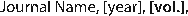
\includegraphics{head_foot/RF}}
\fancyfoot[CE]{\vspace{-7.2pt}\hspace{-14.2cm}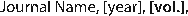
\includegraphics{head_foot/RF}}
\fancyfoot[RO]{\footnotesize{\sffamily{1--\pageref{LastPage} ~\textbar  \hspace{2pt}\thepage}}}
\fancyfoot[LE]{\footnotesize{\sffamily{\thepage~\textbar\hspace{3.45cm} 1--\pageref{LastPage}}}}
\fancyhead{}
\renewcommand{\headrulewidth}{0pt}
\renewcommand{\footrulewidth}{0pt}
\setlength{\arrayrulewidth}{1pt}
\setlength{\columnsep}{6.5mm}
\setlength\bibsep{1pt}
%%%END OF FOOTER%%%

%%%FIGURE SETUP - please do not change any commands within this section%%%
\makeatletter
\newlength{\figrulesep}
\setlength{\figrulesep}{0.5\textfloatsep}

\newcommand{\topfigrule}{\vspace*{-1pt}%
\noindent{\color{cream}\rule[-\figrulesep]{\columnwidth}{1.5pt}} }

\newcommand{\botfigrule}{\vspace*{-2pt}%
\noindent{\color{cream}\rule[\figrulesep]{\columnwidth}{1.5pt}} }

\newcommand{\dblfigrule}{\vspace*{-1pt}%
\noindent{\color{cream}\rule[-\figrulesep]{\textwidth}{1.5pt}} }

\makeatother
%%%END OF FIGURE SETUP%%%

%%%TITLE, AUTHORS AND ABSTRACT%%%
\twocolumn[
  \begin{@twocolumnfalse}
\vspace{3cm}
\sffamily
\begin{tabular}{m{4.5cm} p{13.5cm} }


\includegraphics{head_foot/DOI} & \noindent\LARGE{\textbf{Local Structure and Lithium Ion Diffusion Pathway of Cubic Li$_7$La$_3$Zr$_2$O$_{12}$ Studied by Total Scattering and the Reverse Monte Carlo Method$^\dag$}} \\%Article title goes here instead of the text "This is the title"
\vspace{0.3cm} & \vspace{0.3cm} \\

 & \noindent\large{Haolai Tian,$^{\ast}$\textit{$^{a}$} Martin T. Dove,\textit{$^{b\ddag}$} and Xiang Yang Kong\textit{$^{c}$}} \\%Author names go here instead of "Full name", etc.

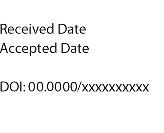
\includegraphics{head_foot/dates} & \noindent\normalsize{ 
The garnet-structured Li$_7$La$_3$Zr$_2$O$_12$ (LLZO)is an excellent candidate for solid electrolytes with its structural stability and high Li+ conductivity. Li+ diffusion path have not yet been thoroughly studied, as well as the precise crystal and local structure. Herein, we use variable-temperature neutron and cynchrotron total scattering in the range of room temperature to 1100 K, and conducte
Reverse Monte Carlo method (RMC) to probe the lithium-ion distribution and framework distortion.
By this analysis, we provide deeper insight into the local structure and Li+ diffusion path of this lithium-ion conductors.
%%
%%The basic perovskite network \textit{AX}$_3$, consisting of corner-linked octahedral groups of atoms,
%has for a long time know to have an inherent flexibility involving rotations of the octahedra. This is often associated with both displacive phase transitions and negative thermal expansion.

} \\

\end{tabular}

 \end{@twocolumnfalse} \vspace{0.6cm}

  ]
%%%END OF TITLE, AUTHORS AND ABSTRACT%%%

%%%FONT SETUP - please do not change any commands within this section
\renewcommand*\rmdefault{bch}\normalfont\upshape
\rmfamily
\section*{}
\vspace{-1cm}


%%%FOOTNOTES%%%

\footnotetext{\textit{$^{a}$~China Spallation Neutron Source (CSNS), Institute of High Energy Physics (IHEP), Chinese Academy of Sciences (CAS), Dongguan 523803, China}}
\footnotetext{\textit{$^{b}$~Centre for Condensed Matter and Materials Physics, School of Physics and Astronomy, Queen Mary University of London, Mile End Road, London, E1 4NS, United Kingdom; E-mail: martin.dove@qmul.ac.uk}}
\footnotetext{\textit{$^{c}$~School of Materials Sciences and Engineering, Shanghai Jiao Tong University, Huashan Road 1954, Shanghai 200030; E-mail: xykong@sjtu.edu.cn}}

%%Please use \dag to cite the ESI in the main text of the article.
%%If you article does not have ESI please remove the the \dag symbol from the title and the footnotetext below.
%\footnotetext{\dag~Electronic Supplementary Information (ESI) available: [details of any supplementary information available should be included here]. See DOI: 00.0000/00000000.}
%%additional addresses can be cited as above using the lower-case letters, c, d, e... If all authors are from the same address, no letter is required

%\footnotetext{\ddag~Additional footnotes to the title and authors can be included \textit{e.g.}\ `Present address:' or `These authors contributed equally to this work' as above using the symbols: \ddag, \textsection, and \P. Please place the appropriate symbol next to the author's name and include a \texttt{\textbackslash footnotetext} entry in the the correct place in the list.}


%%%END OF FOOTNOTES%%%

%%%MAIN TEXT%%%%
\section{Introduction}

Lithium ion batteries have wide application on electric vehicles, mobile devices, and battery
farms for renewable energy storage.  However the commonly used liquid-based electrolytes have
disadvantages such as flammability, volatile  and operating temperature limitations.
Although all-solid-state lithium ion batteries (SSLBs) which are expected to enhance the safety
reliability and performance issues have been long sought, the conductivity of solid electrolytes can not
keep competing at the level of the existed liquid-based counterpart. Most solid electrolytes required both high Li+ conductivity and negligible electronic
conductivity have either high ionic conductivity or high electrochemical stability, which are not suitable for commercialized battery applications.
 Recently the garnet-structured
 Li$_7$La$_3$Zr$_2$O$_12$ (LLZO)\cite{ANIE:ANIE200701144} has attracted much attention as a poential solid electrolytes, which possessed high Li+ conductivity, stability against chemical
reaction with Li metal, moisture, air, as well as a wide potential window. However, LLZO exhibits two phases\cite{ic101914e}
cubic and tetragonal, which represent different Li+ conductivity. The conductivity of the cubic
phase is two orders of magnitude higher than tetragonal one, $~3\times 10^{-4} S/cm$\cite{ANIE:ANIE200701144}
and $~1.63\times 10^{-6} S/cm$\cite{AWAKA20092046}, seperately.
This difference may be related to the distances between Li sites, disorder degree of Li atom, and isotropic diffusion pathways in the cubic phase.
A cubic garnet structure can be described\cite{CUSSEN2011470} as A$_3$B$_3$C$_2$O$_{12}$ array, that La occupies B sites in 8 oxygen coordinated, Zr occupies orctahedral C,
and Li occupies A in tetrahedral coordination. The B$_3$C$_2$O$_{12}$ structure \cite{doi:10.1246/cl.2011.60} is a host framework that contains the A-sited Li (labeled Li1) and additional
unoccupied Li (labeled Li2) in disorted octahedral coordination. A Li diffusion loop is constructed by Li1 and Li2 sites, and forms the 3-D Li+ diffusion pathway connected by
shared Li1 site.

\section{Experimental methods}

\subsection{Synthesis}
The precursor materials used was anhydrous LiOH (Alfa Aesar 99.5\%, dried at 200~$^{\circ}C$ overnight; 10 wt.\% excess was taken to compensate for the loss of lithium under annealing conditions), La2O3 (Alfa Aesar, treated at 950~$^{\circ}C$ overnight), ZrO2 (Alfa Aesar, 99.7\%). The reactants were mixed with a mortar and pestle before reacting them at 950~$^{\circ}C$ for 12 hours. The resultant product was reground and pressed into pellets. The pellets were transferred to an alumina crucible and buried with mother powder, followed by sintering at 1140~$^{\circ}C$ for 20 hours to form single-phase material. The resulting pellets were grounded into powder and stored in an Ar-filled glovebox (<0.1 ppm O2, <0.1 ppm H2O) to prevent reaction with humidity.


\subsection{Neutron Powder Diffraction and Total Scattering}

Neutron powder diffraction and total scattering data were obtained at a number of temperatures on the GEM diffractometer at the
ISIS spallation neutron source, Rutherford Appleton Laboratory, UK. The LLZO sample was contained in a cylindrical thin-walled vanadium can of 8 mm diameter.
This was mounted in a standard vanadium-foil furnace for measurements at and above room temperature (at 293K, 450K, 600K, 750K,
900K and 1100K). Data were collected on six separate occasions, counting for between 5 and 6 hours per temperature.
Measurements were also performed on an empty vanadium can, the empty instrument, and an 8 mm diameter vanadium rod for normalisation and background subtraction.
Those data were processed by the GudrunN software to obtain scattering data $I(Q)$ and PDF data $D(r)$  with a maximum momentum transfer of $Q_{max}$ of 50 \AA$^{-1}$.
Diffraction data were also corrected and reduced using Mantid, and Rietveld analysis was performed by GSAS software.

\begin{figure}[t]
\begin{center}
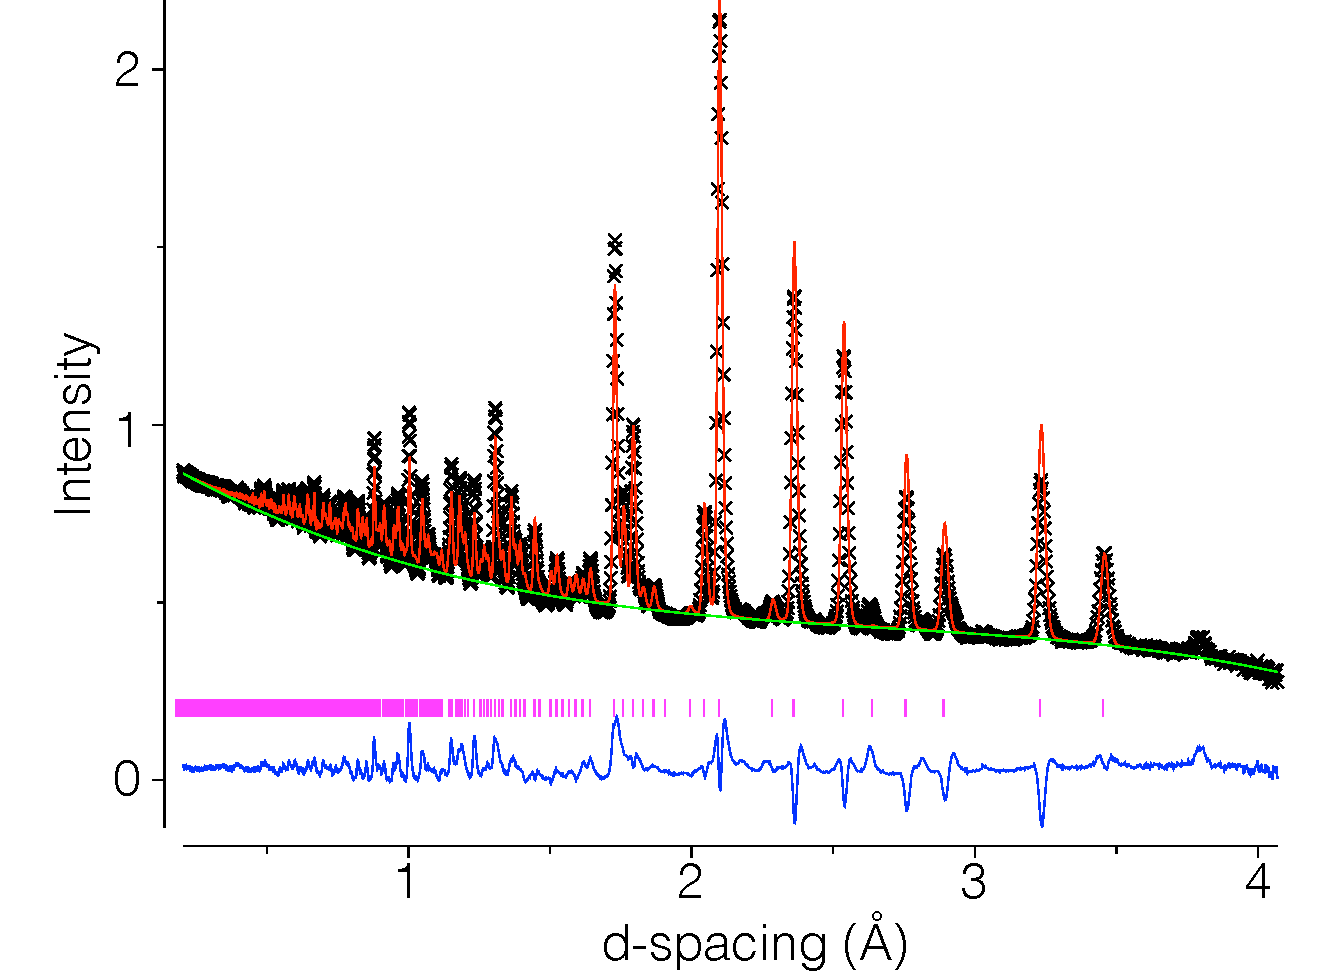
\includegraphics[width=0.4\textwidth]{Pics/gsas.pdf}
\caption{Example of the quality of the Rietveld refinement of the crystal structure
 of LLZO from data collected from the $60^o$ (Bank 4) at temperature of 293K.}
\label{fig:gsas}
\end{center}
\end{figure}

\subsection{Synchrotron  Total Scattering}
Synchrotron powder diffraction and total scattering data were collected on the XPDF beamline (I15-1 instrument) at Diamond Light Source (UK).
The X-rays were monochromatized to yield a wavelength of 0.161669~\AA.
%PerkinElmer XRD 16611 CP3 and a PerkinElmer XRD 4343 CT were used as primary and secondary detectors.
The sample was sealed into borosilicate capilaries ($\phi$ 1 mm, and 50 mm in length) for measurements at and above room temperature
(at 295K, 450K, 600K, 750K, 900K, and 1100K).
The raw data  were corrected and reduced into scattering data using the program DAWN \cite{S1600577515002283}.
And PDF $D(r)$ were processed from scattering data using GudrunX with Q-range 0.5 $\le$ Q $\le$ 25 \AA$^{-1}$ for the Fourier transformation.
The fluorescence corrections were applied, in which the fluorescence energy of La was assumed to be 38.739 keV.

\begin{figure}
\centering
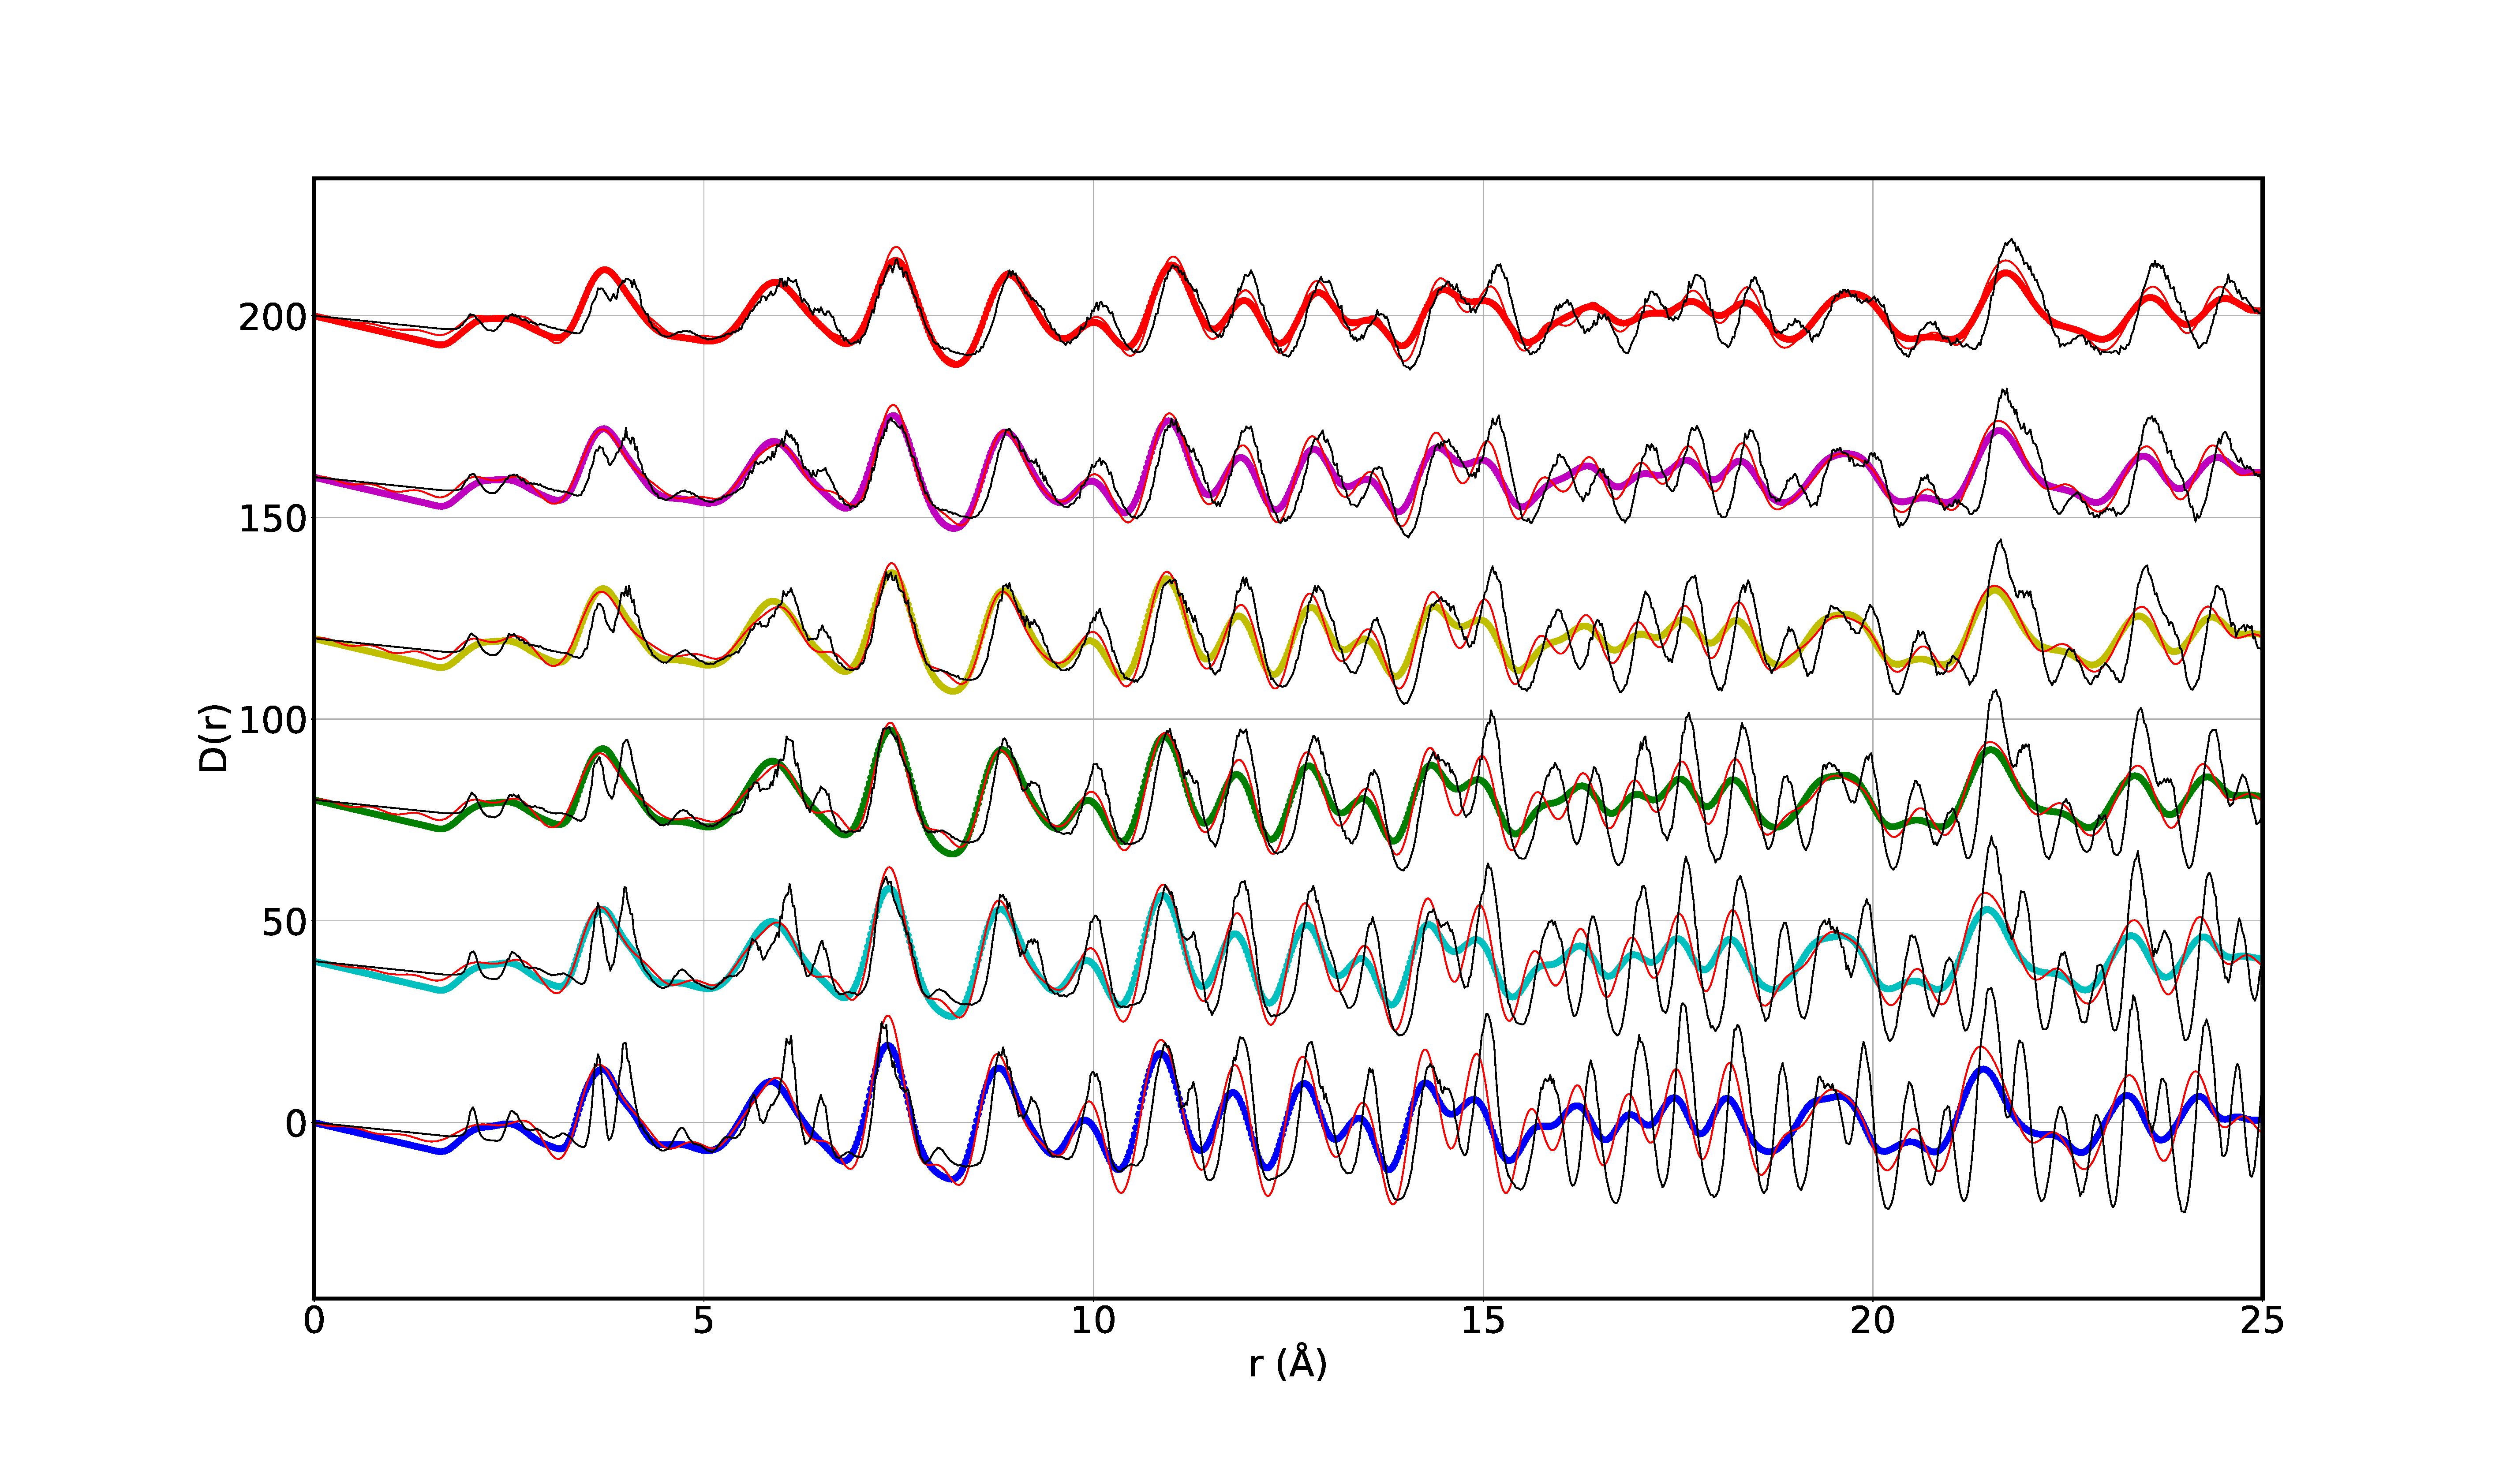
\includegraphics[width=0.5\textwidth]{Pics/xpdf.pdf}
\caption{Synchrotron pair distribution $D(r)$ obtained from GudrunX for all temperatures represented as circles.
 A constant offset has been applied to separate those curves.
 The solid black lines indicate the  simulated intensities from Dl\_poly, and RMC modeling are represented by the solid red lines.
 }
\label{fig:xpdf}
\end{figure}

\subsection{Pair Distribution Function (PDF)}
In the diffraction theory, the differential cross section is defined as

\begin{equation}
\frac{1}{N}\frac{d\sigma}{d\Omega}=I(Q)=I^{S}(Q)+i(Q)
\end{equation}

where $I^{S}(Q)=\sum_{i=1}^{n}c_i\frac{\sigma_{i}}{4\pi}$ is the self-scattering of all atoms,
and $i(Q)$ is the total scattering structure factor in which we are interested. Here we define partial pair
distribution function $g_{mn}(r)$ to present the number of atoms of type $n$ within the shell between $r$ and  $r+dr$ centered on a particle of type $m$.
And then the structure factor $i(Q)$ can be presented as

\begin{equation}
i(Q)=4\pi\rho\int^{\infty}_{0}\sum_{m,n}c_m c_n b_m b_n r^2 [g_{mn}(r)-1]\frac{\sin{Qr}}{Qr}dr
\end{equation}

where $c_m$, $b_m$, and $\rho$ denote the fraction of atoms of type $m$, the  scattering length of species $m$, and the average atomic number density.
Overall pair distribution function is defined as

\begin{equation}\label{fun:dofr_0}
D(r)=4\pi\rho r \sum_{m,n}c_m c_n b_m b_n [g_{mn}(r)-1]
\end{equation}

The $D(r)$ can be calculated via Fourier transformation of $i(Q)$

\begin{equation}\label{fun:dofr_1}
D(r)=\frac{2}{\pi}\int^{Q_{max}}_{0} M(Q)Qi(Q)\sin{Qr}dr
\end{equation}

where $M(Q)$ is the Lorch function to reduce the effect of finite maximum momentum transfer, $Q_{max}$. Those tasks were carried out using the program GudrunX and GudrunN.


\begin{figure}
\centering
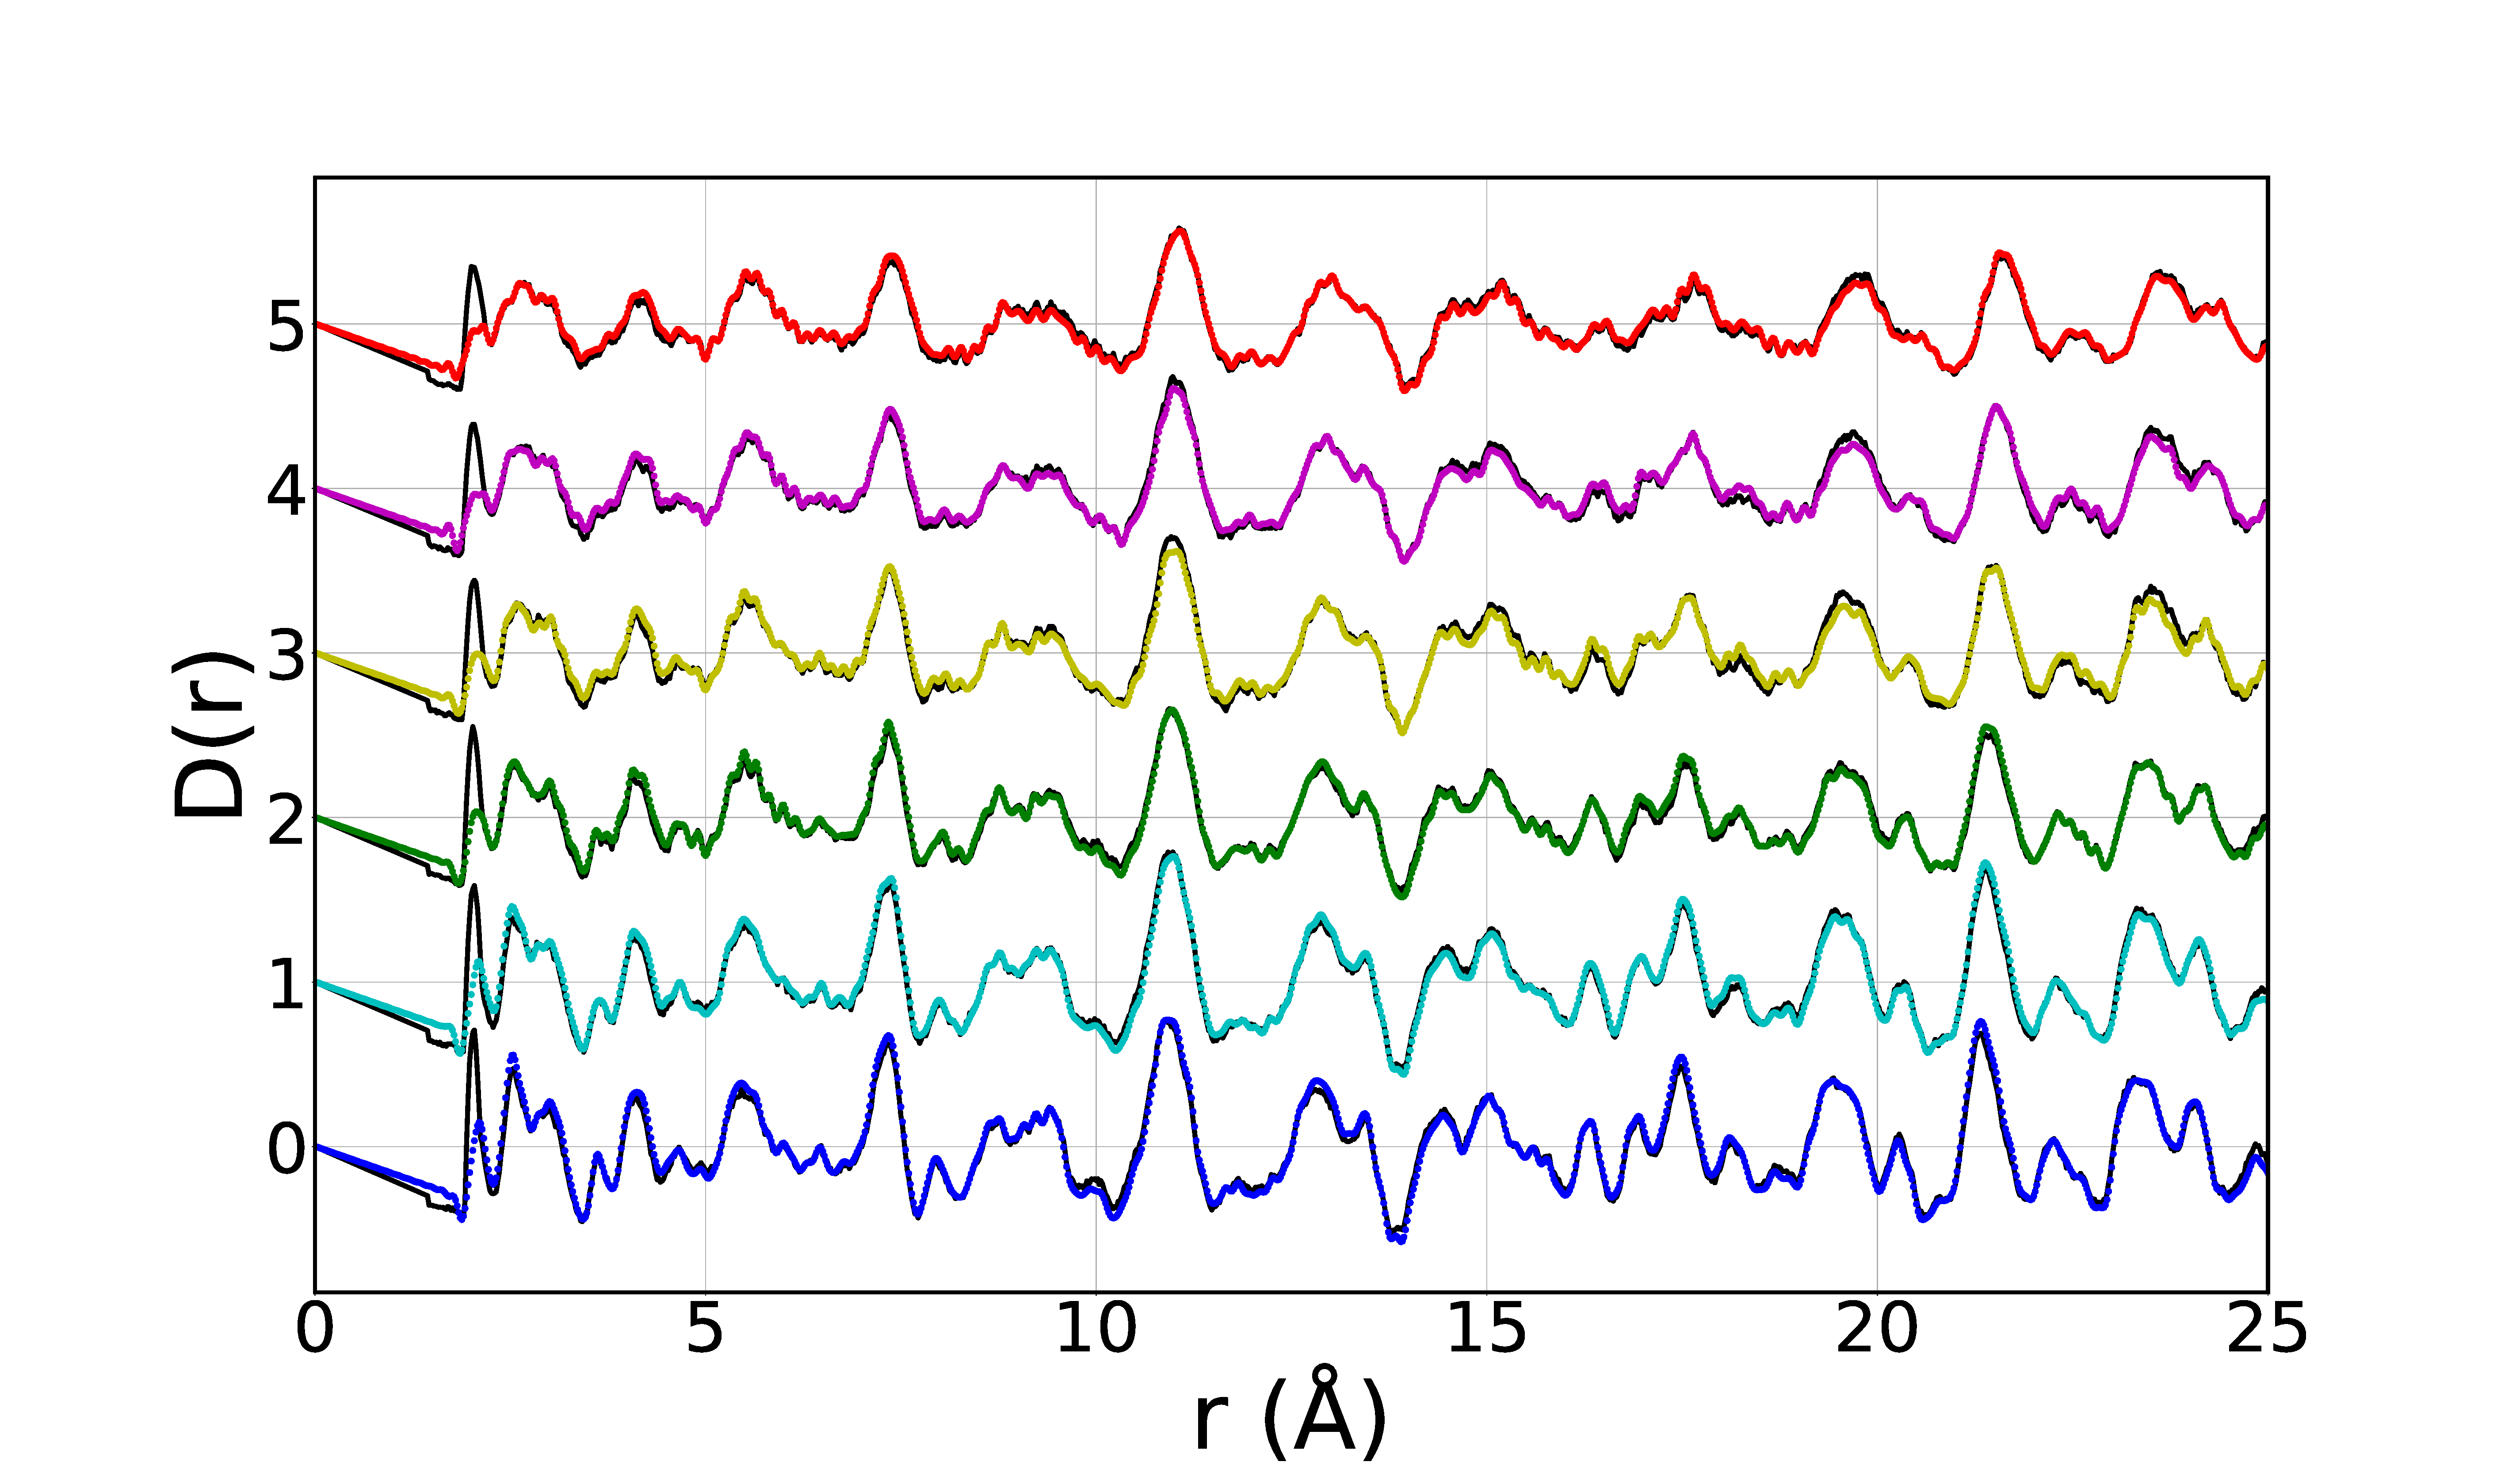
\includegraphics[width=0.5\textwidth]{Pics/npdf.pdf}
\caption{Neutron pair distribution $D(r)$  obtained from GudrunN for all temperatures represented as circles.
 A constant offset has been applied to separate those curves.
 The solid black lines indicate the  simulated intensities from Dl\_poly, and RMC modeling are represented by the solid red lines. }
\label{fig:npdf}
\end{figure}

\subsection{Reverse Monte Carlo Analysis (RMC)}

Involving measurements of the total neutron and X-ray powder diffraction,
the RMC Profile program combines and fits all the reciprocal $i(Q)$, real-space $D(r)$ data, and the intensities of thr Bragg peaks at the same time.
The explicit use of the Bragg intensities ensures that the RMC refinement gives configurations that have the correct
long-range average structure and symmetry without any exaggeration of the structural disorder.
The traditional Metropolis Monte Carlo algorithm moves atoms randomly to generate new configration.
In order to keep atomic movement within the crystal structure,
maximum atomic moves of La, O and Zr were of size $0.05 \AA$, but those of Li were $0.1 \AA$.
The minimum distances between pairs of atoms are give in Table  \ref{tab:min_dis}.

$\chi^2$ is definded to reflect the agreenment  between calculated (Monte Carlo) and observed (measured) curves

\begin{equation}
\chi^2=\sum_{j}\sum_{i}(y^{obs}_{i,j}-y^{calc}_{i,j})^2/\sigma_{j}
\end{equation}

where $y^{obs}_{i,j}$ is the observed values at data point $i$ in data set $j$, $y^{calc}_{i,j}$ is the calculated counterpart, and  $\sigma_{j}$ is the weighing that represents
the statistical accuracy of data set. In this study, data sets include $i(Q)$ from both neutron and  synchrotron power diffraction, and $D(r)$ and Bragg data from neutron diffraction only,
all with equal $\sigma_{j}$. An atomic move can be accepted when the value of $\chi^2$ declines. If the value of $\chi^2$ raises by $\Delta \chi^2$, the probability of accception is $exp(-\Delta \chi^2/2)$

\begin{figure}
\centering
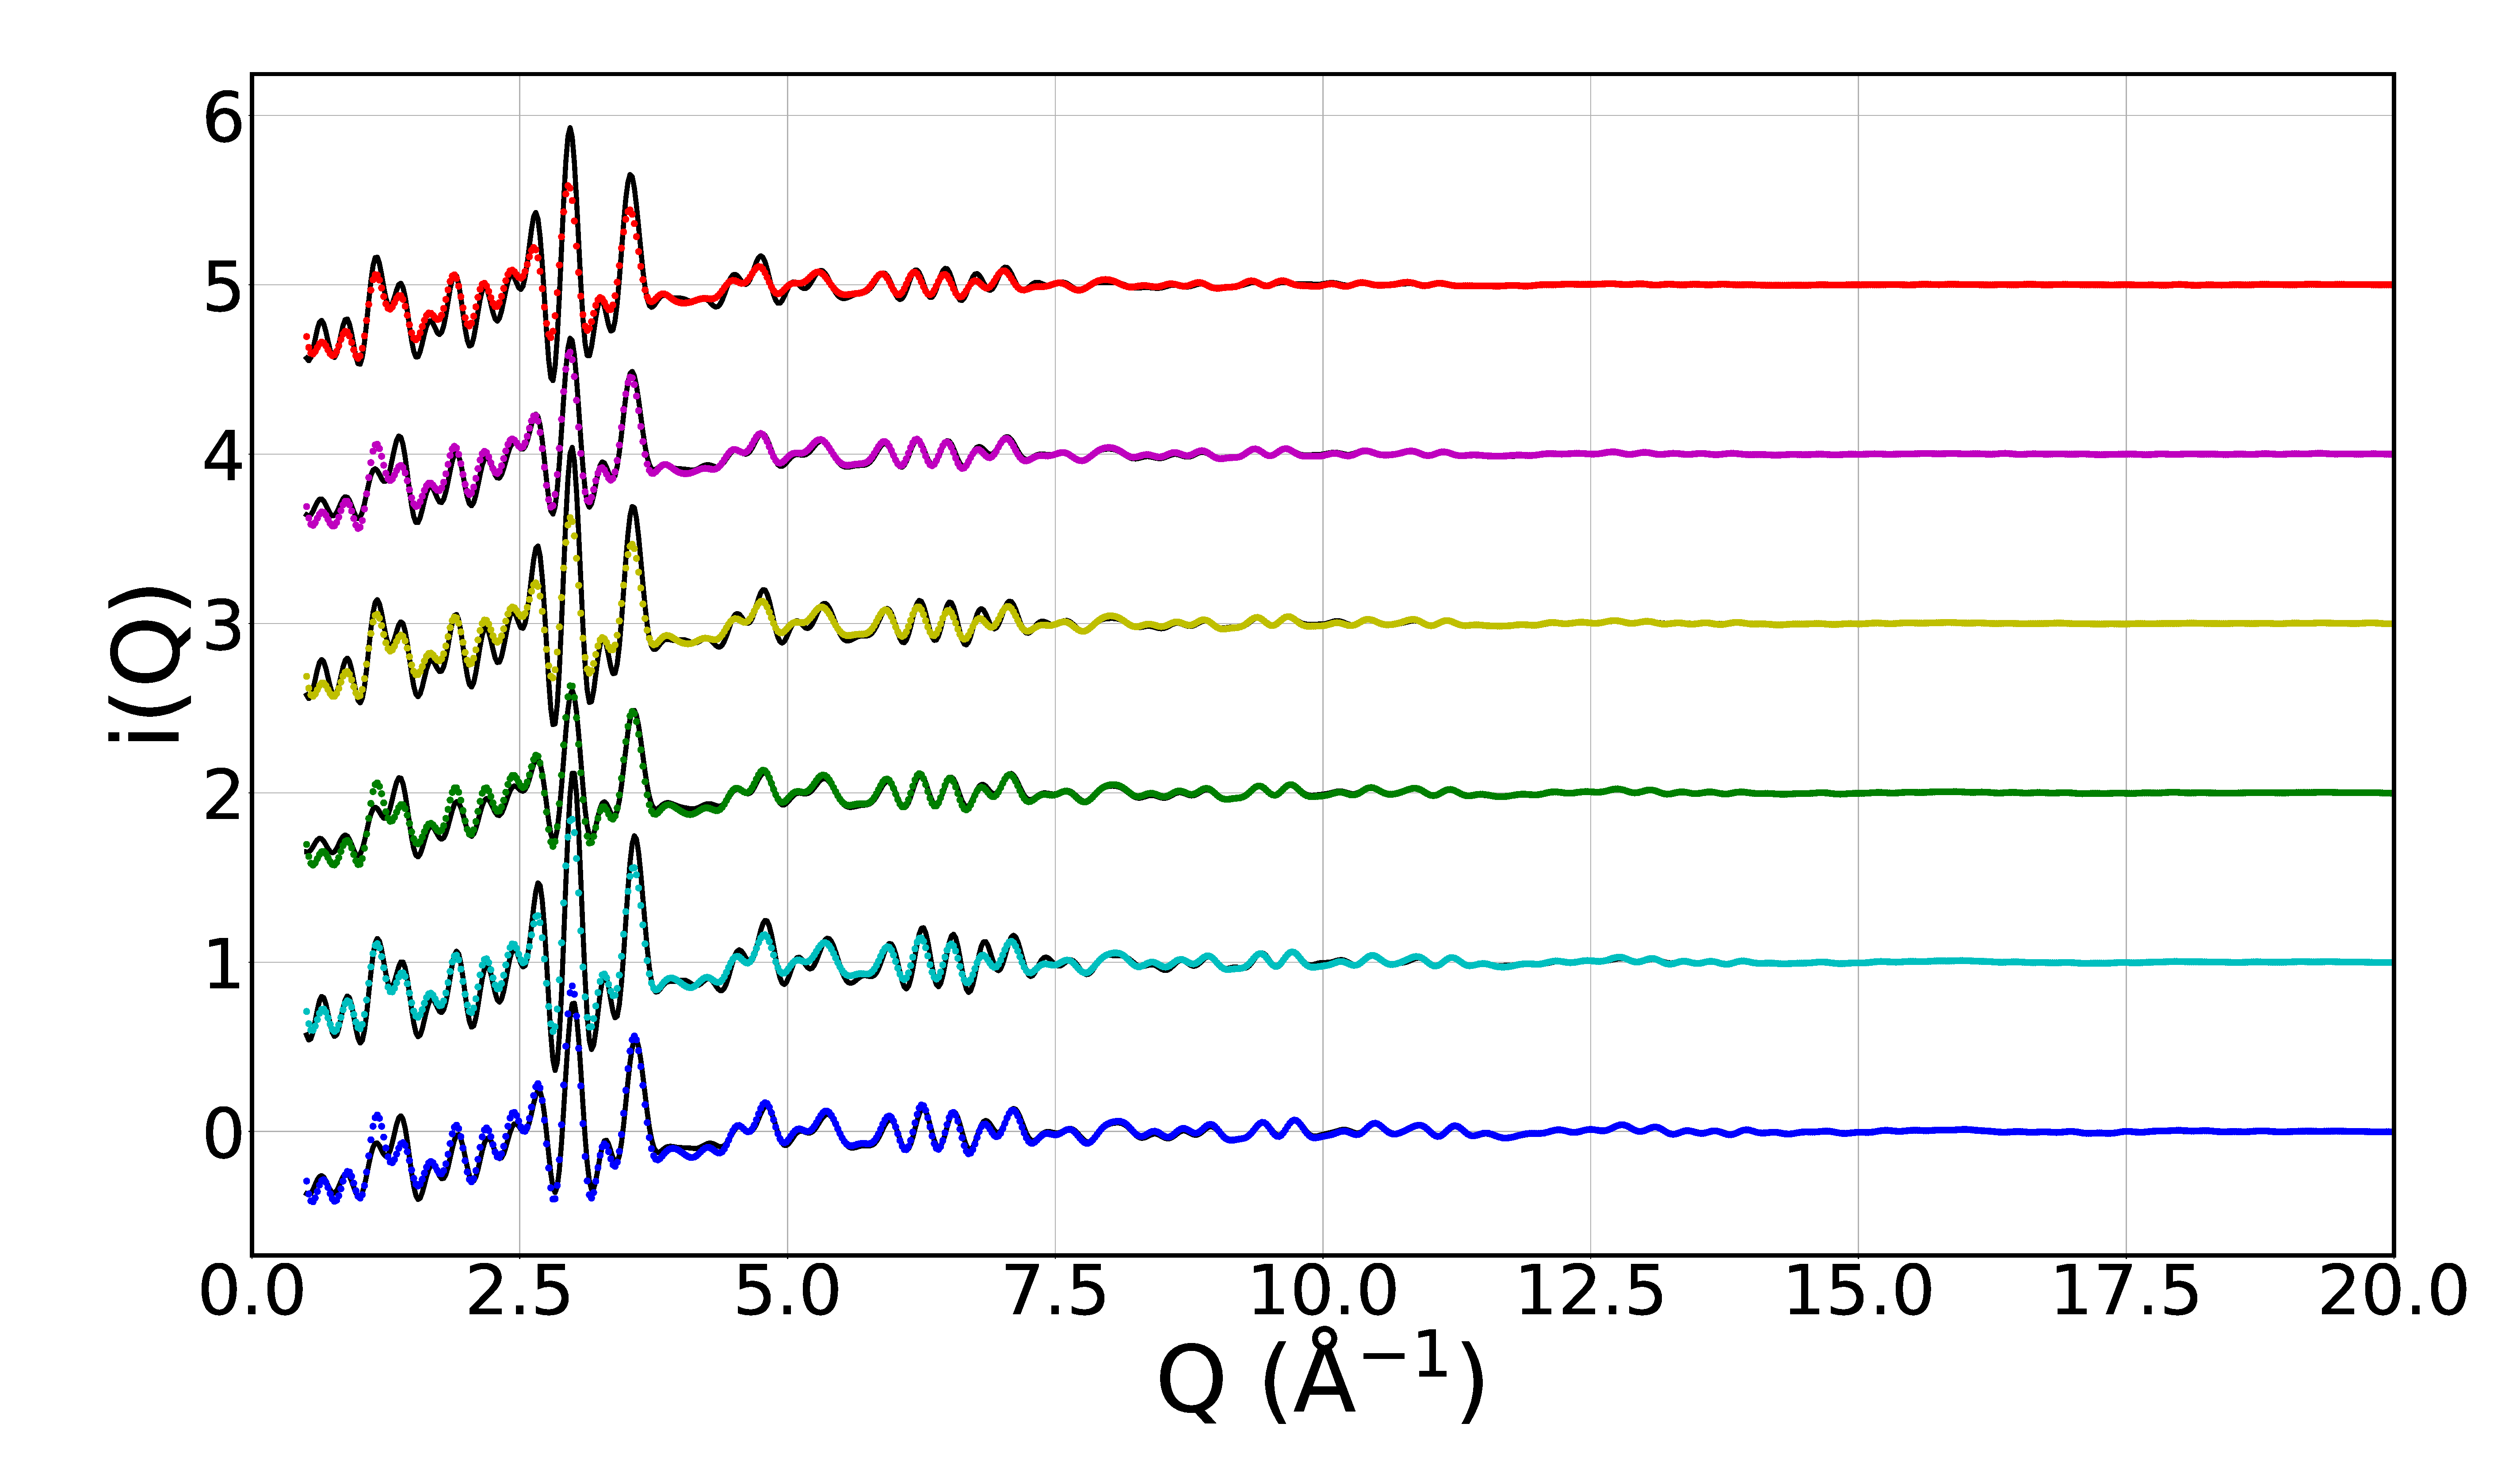
\includegraphics[width=0.5\textwidth]{Pics/nsoq.pdf}
\caption{Neutron scattering function $S(Q)$ for all temperatures. A constant offset has been applied to separate those curves.}
\label{fig:nsoq}
\end{figure}

The initial RMC configuration were generated from the crystal strucutres got by Rietveld refinement of neutron diffraction.
Each contained $4\times 4\times 4$ unit cells with 12288 atoms. And the RMC analysis were run for long enough to ensure the convergence of the simulation by checing the value of $\chi^2$.



\begin{table}[h]
\centering
\caption{The minimum distances between pairs of atoms} \label{tab:min_dis}
\begin{tabular}{c|cccc}
\hline
   & Li & O & Zr & La \\
\hline
Li & 1.69 & 1.50 & 2.3 & 2.3 \\
O  &      & 2.2  & 1.79& 2.2 \\
Zr &      &      & 5.0 & 3.3 \\
La &      &      &     & 3.3 \\
\hline
\end{tabular}
\end{table}

\subsection{Electrochemical Impedance Measurements}

Electrochemical experiments were carried out in an Ar glovebox (O$_2$; H$_2$O < 1 ppm). For the electrical measurement, 
gold electrodes were evaporated on LLZO by thermal evaporation. The EIS was recorded by a Solartron ModuLab system, 
and contacted via a probe station on a hot stage in the glovebox. EIS was performed with an 10 mV amplitude voltage 
in a frequency range of 50 mHz to 1 MHz.

\subsection{Molecular Dynamic Simulation (MD)}
Classical MD simulations were performed on $4\times 4\times 4$ unit cells and 12288 atoms of LLZO using the DL\_POLY package.
Empirical force-fields similar to previous work were employed which include the long-range Coulombic potential,
short-range Buckingham potential, and Dick-Overhauser core-shell potential for O atoms.
The parameters of force-field are listed in Table \ref{tab:md_force}.
Constant number, volume, and energy (NVE) ensemble simulations were carried out at 300K, 450K, 600K, 750K, 900K and 1100K.
Each initial configurations came from the result of RMC analysis at same temperature.
The simulations were performed for 10 ps with atomic positions saved every 0.01 ps.



%\begin{table}[h]
%\centering
%\caption{Force-field parameters} \label{tab:md_force}
%\begin{tabular}{cccccc}
%\hline
%      & \multicolumn{3}{c}{Buckingham parameters}    & \multicolumn{2}{c}{O shell parameters}         \\
%\hline
%      & A (eV)  & $\rho$(\AA) & C(eV\AA$^6$)         &                    &       \\
%Zr-O  & 1385.02 & 1.79        & 0                    & Y (e)              &  -2.76\\
%La-O  & 4579.23 & 0.3044      & 0                    & k (eV $\AA^{-2}$)  &  30.2 \\
%Li-O  & 632.102 & 0.2906      & 0                    & m (au)             &  0.2  \\
%O-O   & 22764.30& 0.1490      & 27.63                &                    &       \\
%\hline
%\end{tabular}
%\end{table}

\begin{table}[h]
\centering
\caption{Force-field parameters} \label{tab:md_force}
\begin{tabular}{cccccc}
\hline
      & \multicolumn{3}{c}{Buckingham parameters}      \\
\hline
      & A (eV)  & $\rho$(\AA) & C(eV\AA$^6$)           \\
Zr-O  & 1385.02 & 1.79        & 0                      \\
La-O  & 4579.23 & 0.3044      & 0                      \\
Li-O  & 632.102 & 0.2906      & 0                      \\
O-O   & 22764.30& 0.1490      & 27.63                  \\
\hline
\end{tabular}
\end{table}

\begin{figure}
\centering
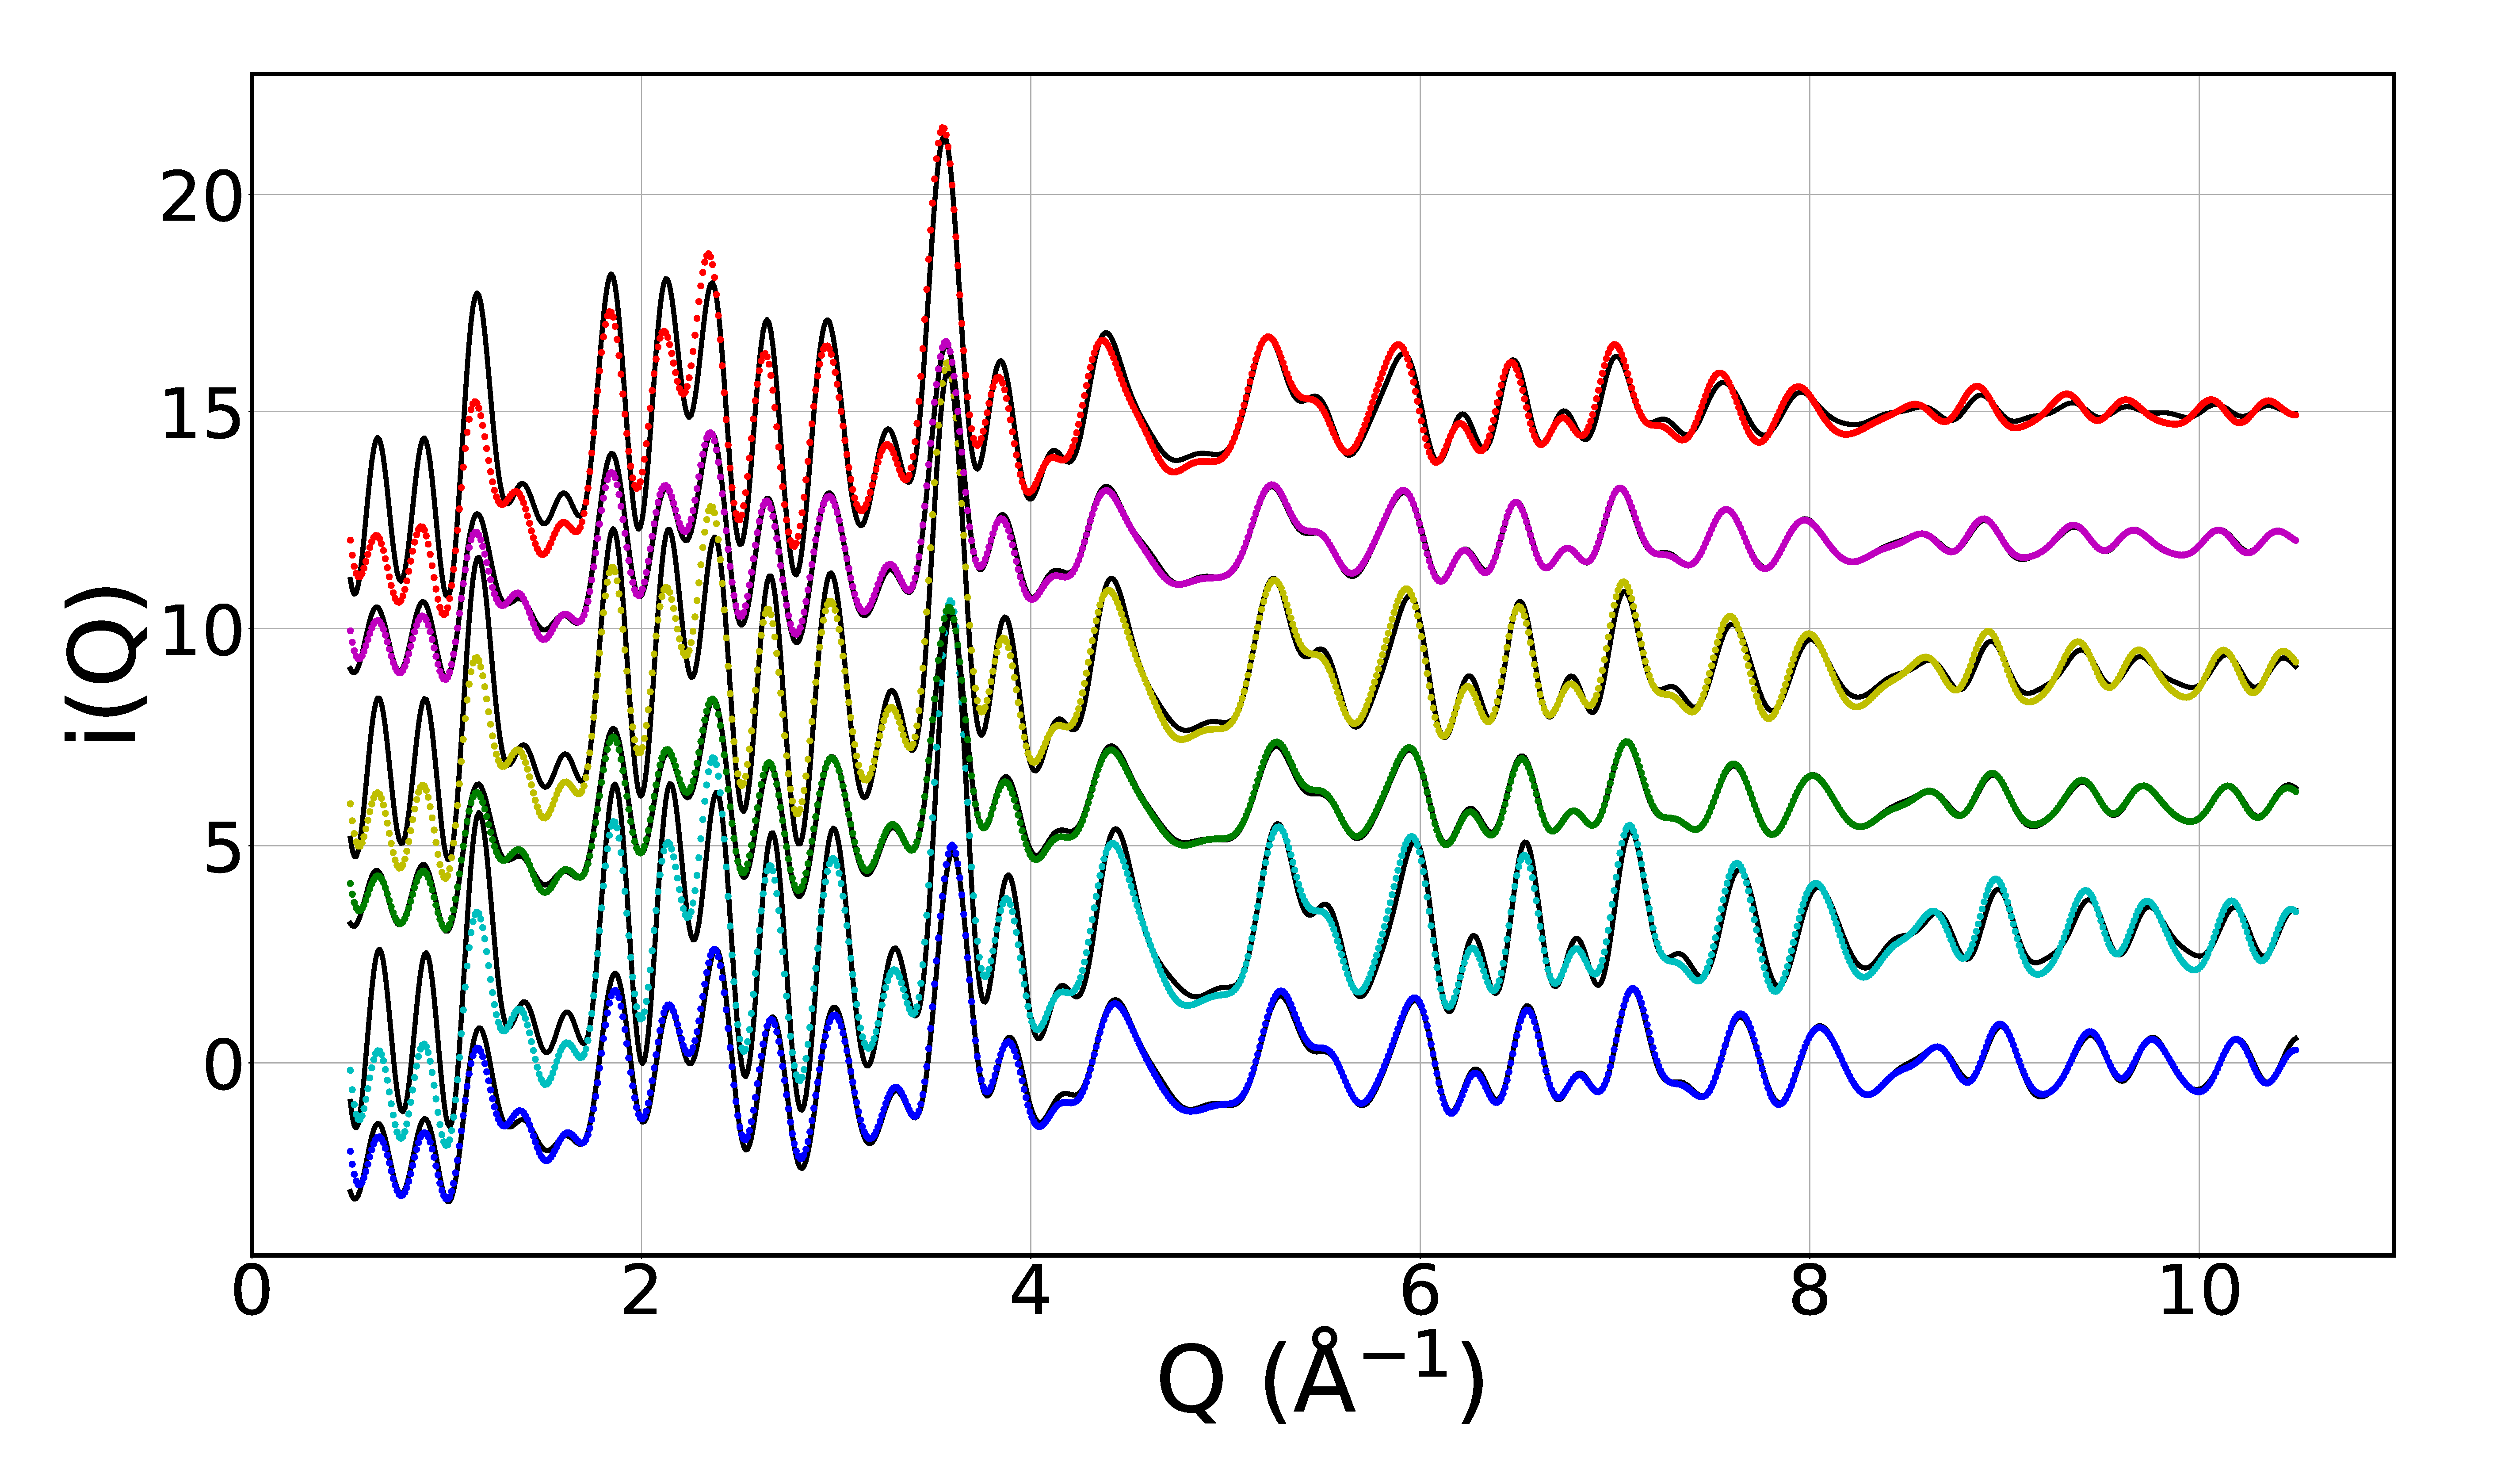
\includegraphics[width=0.5\textwidth]{Pics/xsoq.pdf}
\caption{Synchrotron scattering function $S(Q)$ for all temperatures. A constant offset has been applied to separate those curves.}
\label{fig:xsoq}
\end{figure}




%\subsection{GASP analysis}
%
%Both our RMC and MD configurations have been analysed using the GASP method. 
%In this method the motions of the atoms associated with each polyhedron in 
%the configuration are described together as a combination of whole-polyhedron rotation, 
%bond-bending and bond-stretching motions.


\section{Results and discussion}
\subsection{Crystal Structure Analysis}

The structural parameters of Rietveld refinement for all temperatures are listed in Table \ref{tab:cell_parameters},
which fitted well to the cubic model with space group $Ia\bar{3}d$. A sample fit to the data, namely for the data at 293K, is shown in Fig.\ref{fig:gsas}
The lattice parameters are plotted as functions of temperature in Fig.\ref{fig:lattice}, showing a linear thermal expansion.


\begin{table*}[h]
\centering
\caption{Cell parameters and atomic fractional coordinates of LLZO. Zr has fractional coordionals 0,0,0, La has fractional coordinations 0.125,0,0.25, and Li1 has fractional coordinations 0.25,0,0.125. } \label{tab:cell_parameters}
\begin{tabular}{cccccccc}
\hline
\hline
T(K)  & a(\AA)   & $O_{x}$      & $O_{y}$             & $O_{z}$       & $Li2_{x}$      & $Li2_{y}$           & $Li2_{z}$      \\
\hline
273  & 12.921935 & 0.101587    & 0.196351             &0.282562       & 0.125          & 0.174334            & 0.424334       \\
450  & 12.952953 & 0.102189    & 0.196519             &0.281758       & 0.125          & 0.187500            & 0.437500       \\
600  & 12.980208 & 0.102160    & 0.197170             &0.281250       & 0.125          & 0.187500            & 0.437500       \\
750  & 13.009548 & 0.101086    & 0.195999             &0.282573       & 0.125          & 0.172539            & 0.422539       \\
900  & 13.045011 & 0.102160    & 0.197170             &0.281250       & 0.125          & 0.187500            & 0.437500       \\
1100 & 13.086332 & 0.101519    & 0.197491             &0.282502       & 0.125          & 0.177546            & 0.427546       \\
\hline
\hline
\end{tabular}
\end{table*}


\begin{figure}
\centering
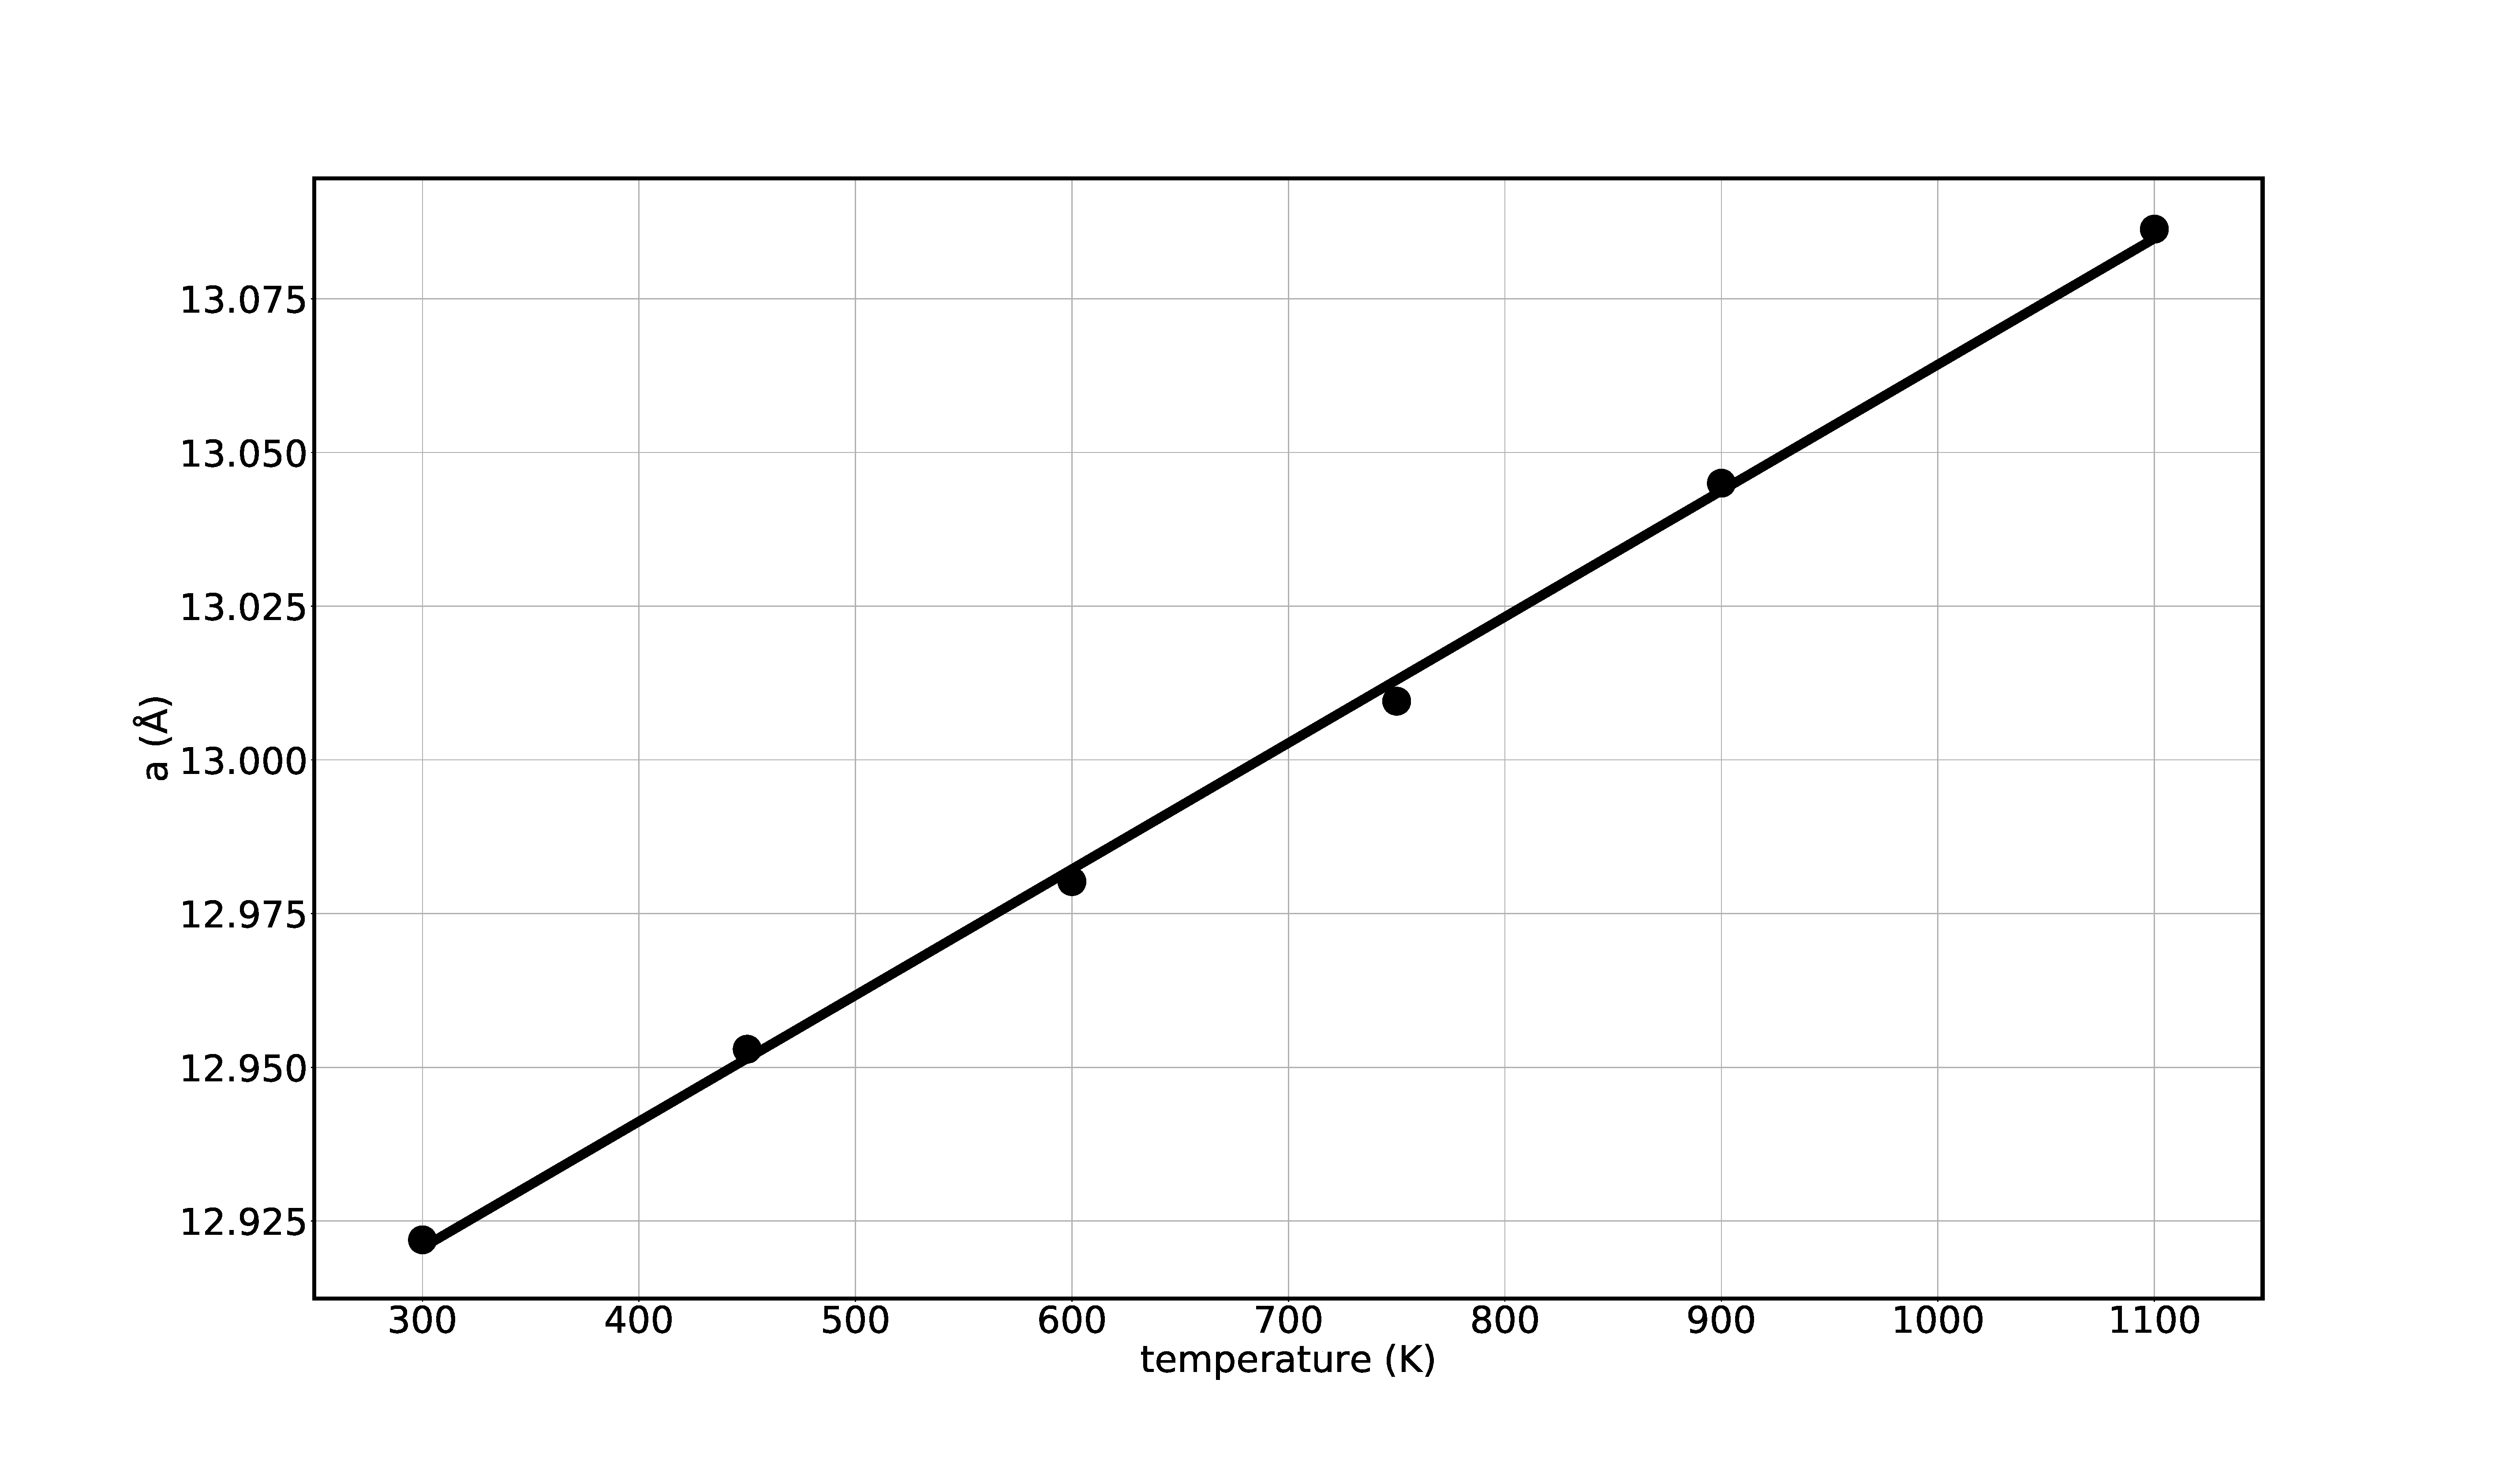
\includegraphics[width=0.5\textwidth]{Pics/lattice.pdf}
\caption{Variation of the lattice parameters with temperature, obtained by Rietveld analysis. }
\label{fig:lattice}
\end{figure}

the average structure calculated from the RMC configurations agreed well with Rietveld refinement, as shown in Fig. \ref{fig:Rietveld_refinement}



\begin{figure}
\centering
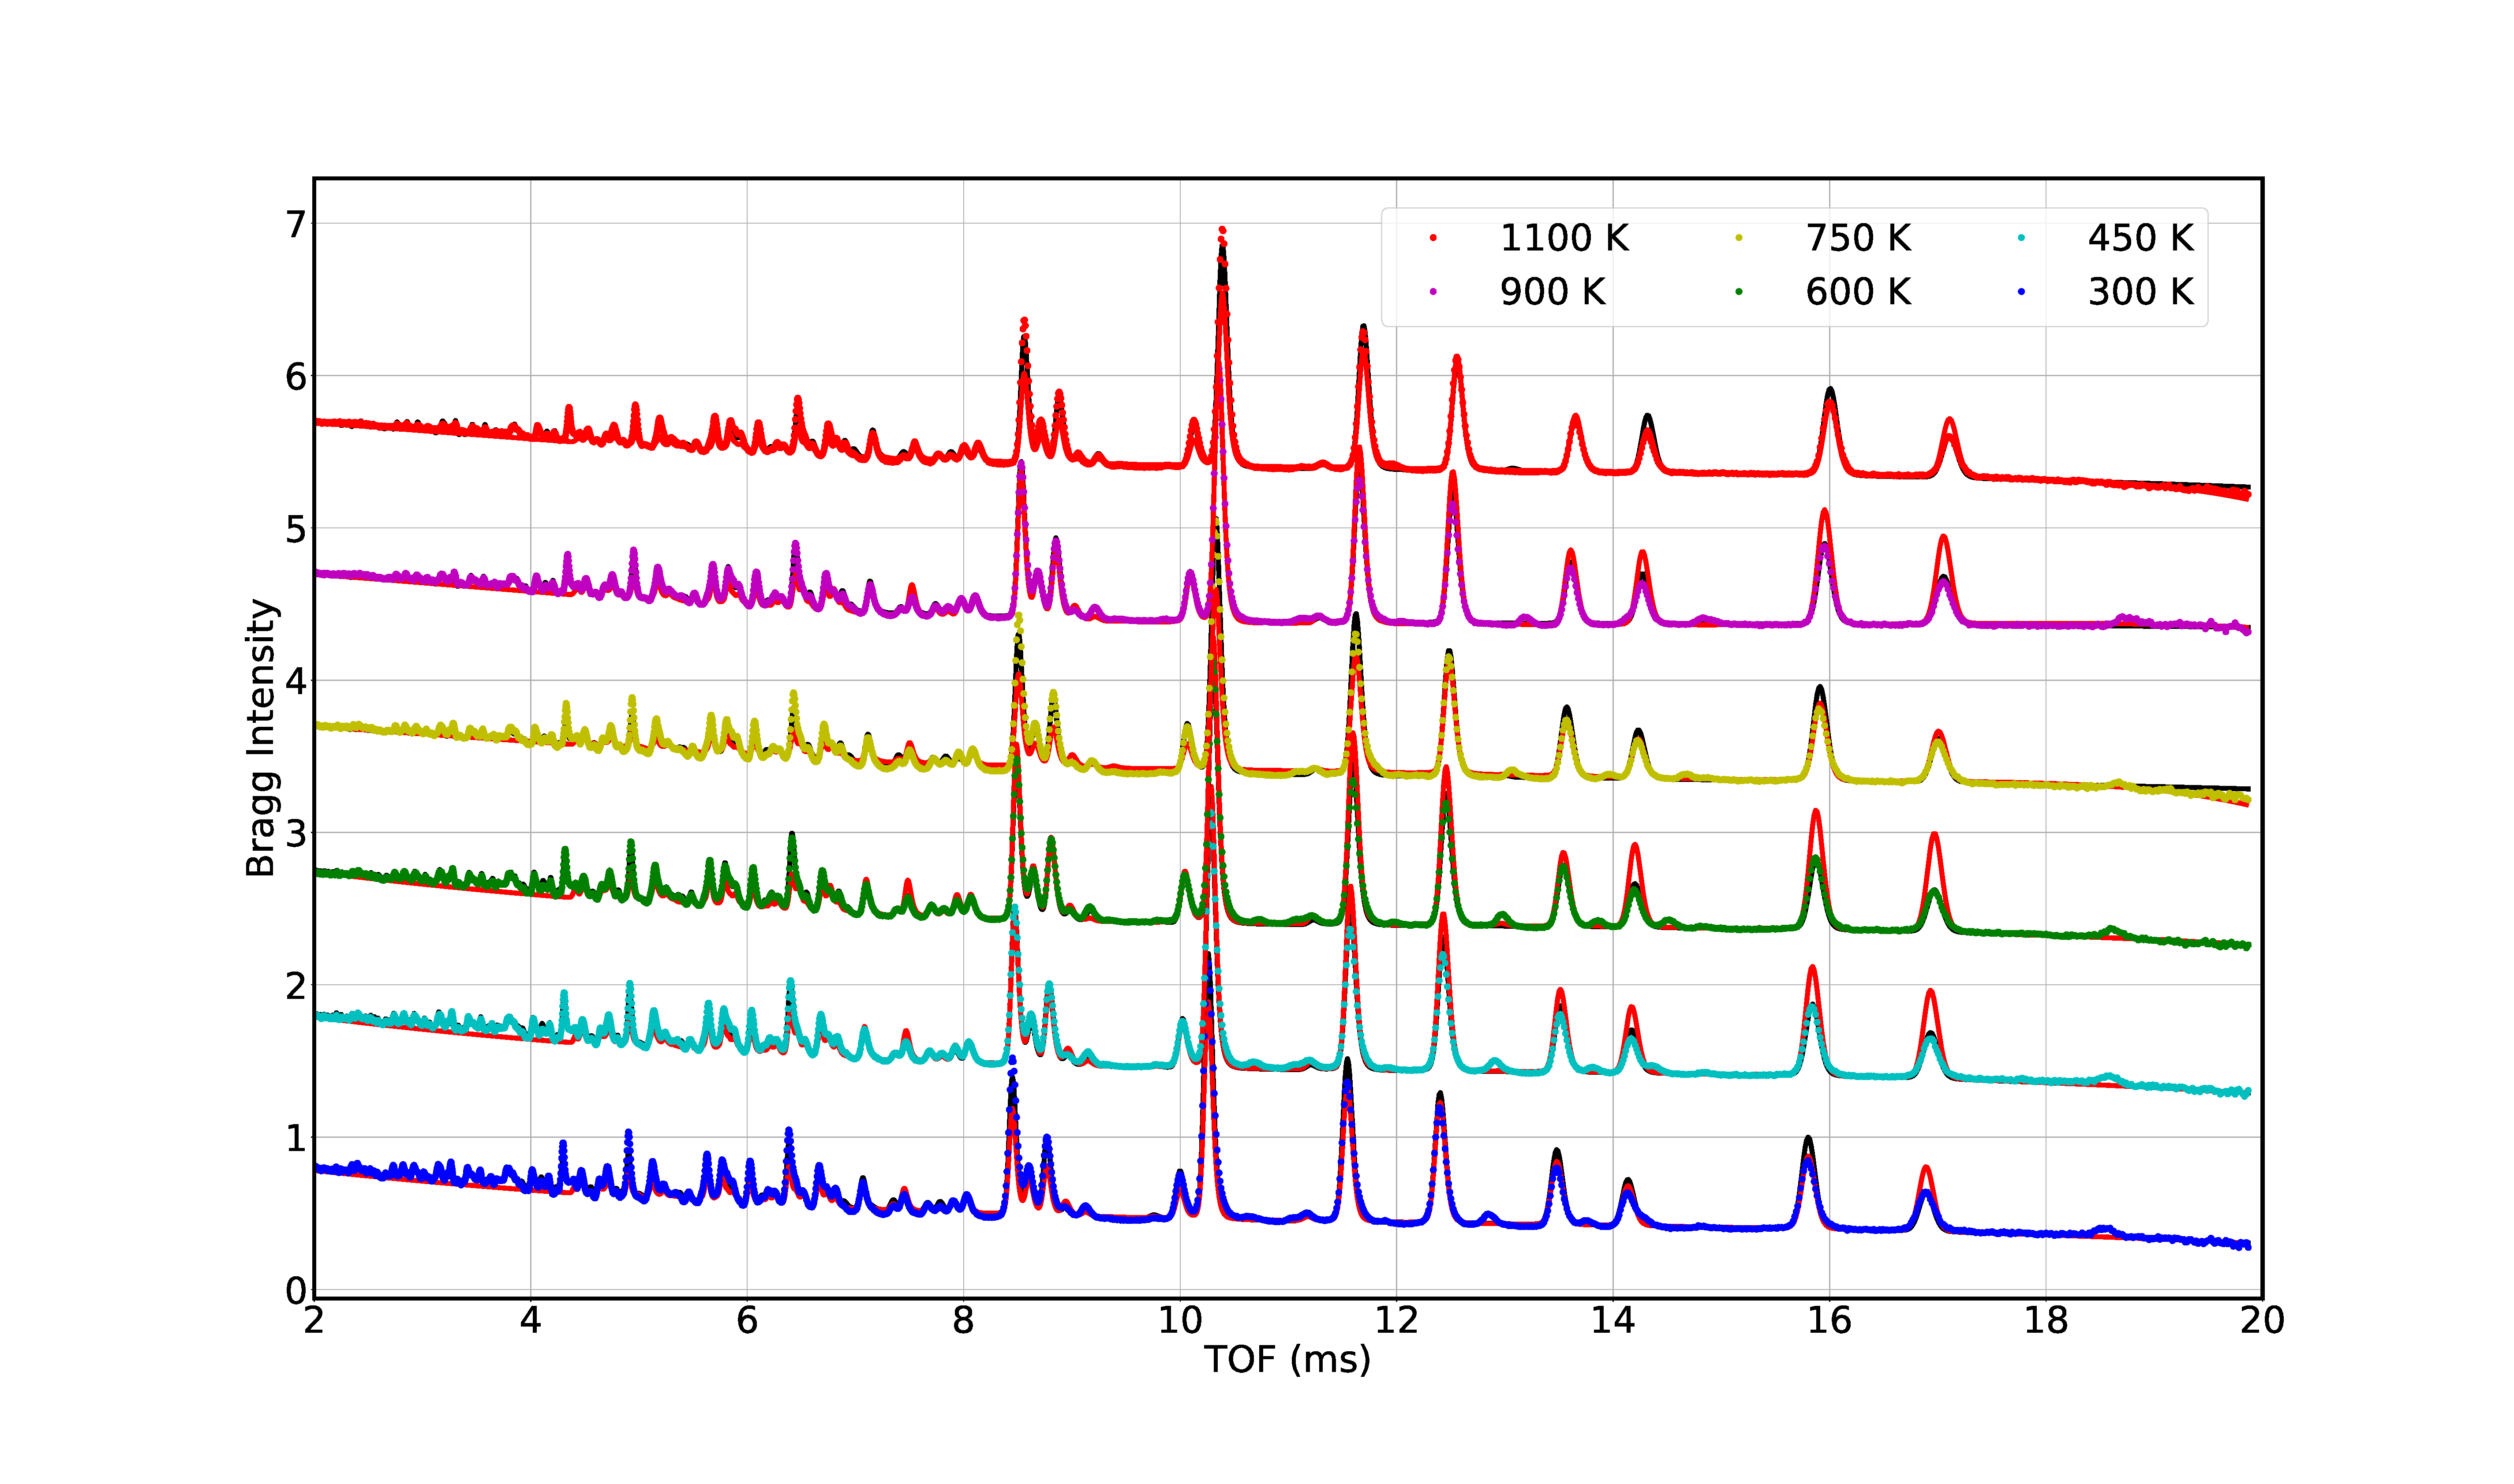
\includegraphics[width=0.5\textwidth]{Pics/bragg.pdf}
\caption{The Bragg diffraction data. The data are represented as circles with constant offset to separate those curves.
The solid black lines indicate the  calculated intensities from GSAS, and RMC modeling are represented by the solid red lines. }
\label{fig:Rietveld_refinement}
\end{figure}

\subsection{Local Structure Analysis}
The synchrotron pair distribution function $D(r)$ defined as functions \ref{fun:dofr_0} and \ref{fun:dofr_1}, are shown in Fig. \ref{fig:xpdf}.
The first peak corresponds to the La-O nearest-neighbor distance at around 2.5~\AA, and the second peaks refers to La-Zr around 3.6~\AA.
The position and integrated area are constant for all temperatures,
reflection there is no significant differences in crystal framwork structure. The higher-$r$ PDF shows shifting and broadening of the peaks as the temperature rising,
because of the increases of the lattice parameters.

 The RMC analysis used 4 data sets to perform RMC fits, including Bragg data (Fig.\ref{fig:Rietveld_refinement}) and PDF $D(r)$ from neutron total scattering (Fig.\ref{fig:npdf}),
 and scattering function $i(Q)$ from both neutron (Fig.\ref{fig:nsoq})  and synchrotron experiments(Fig.\ref{fig:xsoq}) .


The low-$r$  distributions of distances from the RMC and MD configurations are shown in Fig.\ref{fig:partialPDFwithLi} and  Fig.\ref{fig:partialPDFwithoutLi}. The interesting point about these diagrams is that
the Li-X (X represents Li, La, Zr or O) distribution from RMC are smoother than those from MD in all temperatures, as shown in Fig.\ref{fig:partialPDFwithLi}, indicating the Li-ion movement remains  disorderly.
But the framework structure keep stable in each case as shown in Fig.\ref{fig:partialPDFwithoutLi}, which is consist with the result of XPDF as shown in Fig. \ref{fig:xpdf}.




\begin{figure}
\centering
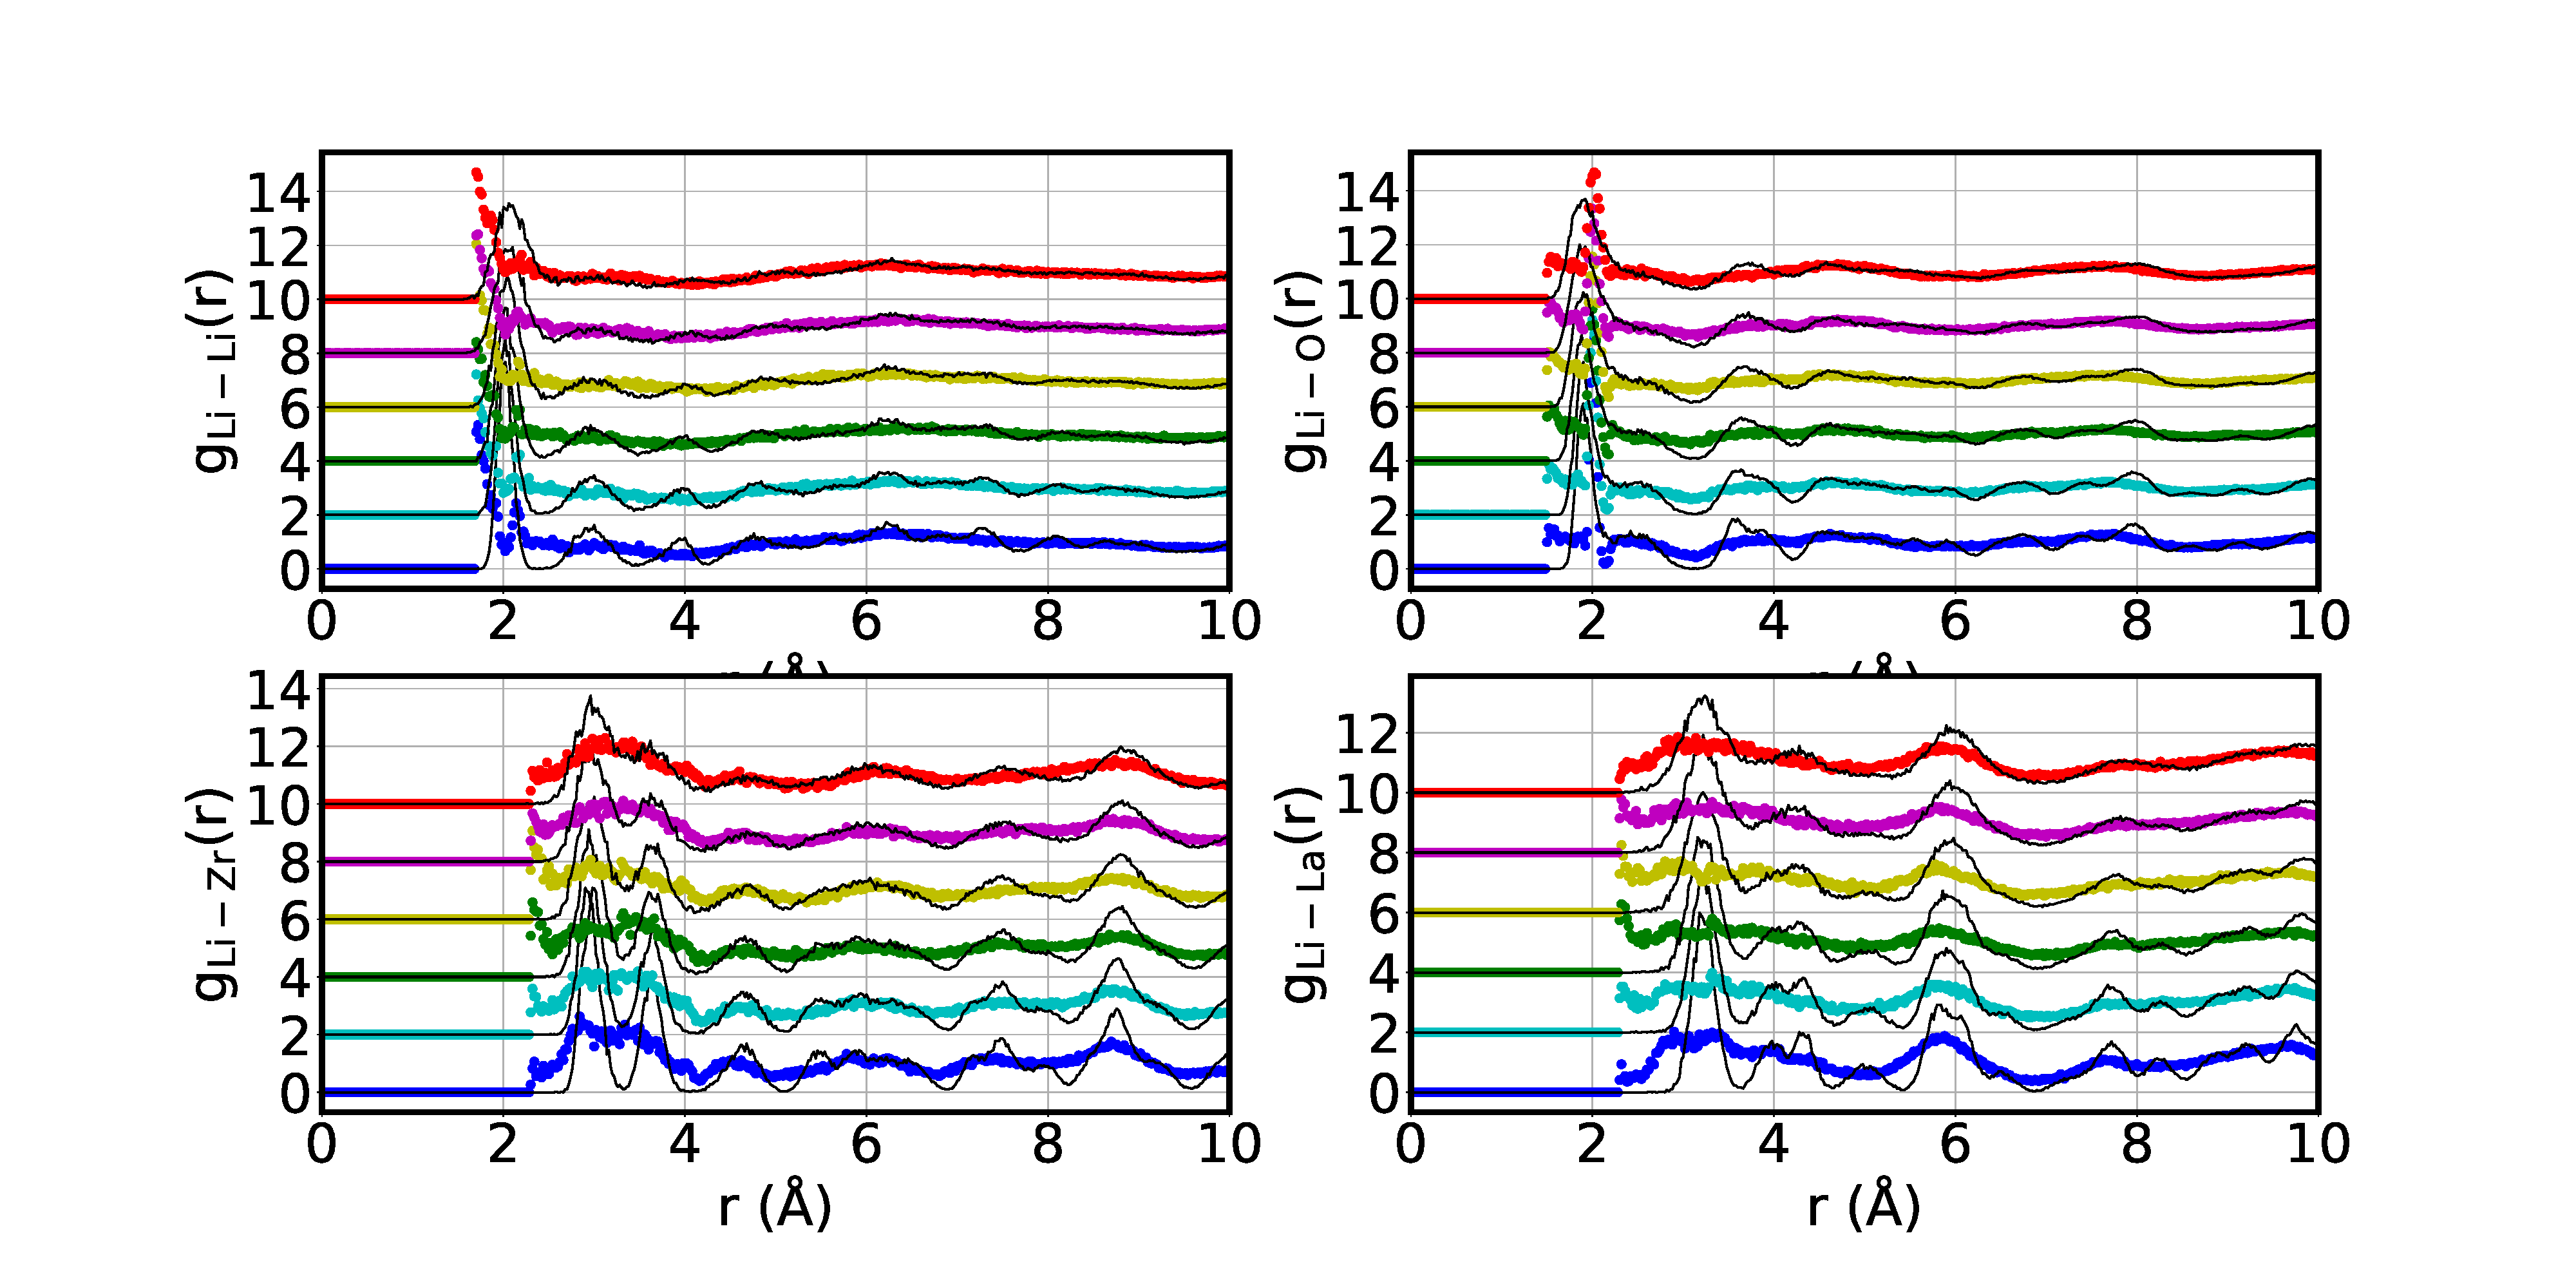
\includegraphics[width=0.5\textwidth]{Pics/partialPDFwithLi.pdf}
\caption{The distributions calculated from RMCProfile of (1) Li-Li, (2)Li-O, (3)Li-Zr, (4)Li-La at low-$r$ range for all temperatures. A constant offset has been applied to separate those curves.}
\label{fig:partialPDFwithLi}
\end{figure}

\begin{figure}
\centering
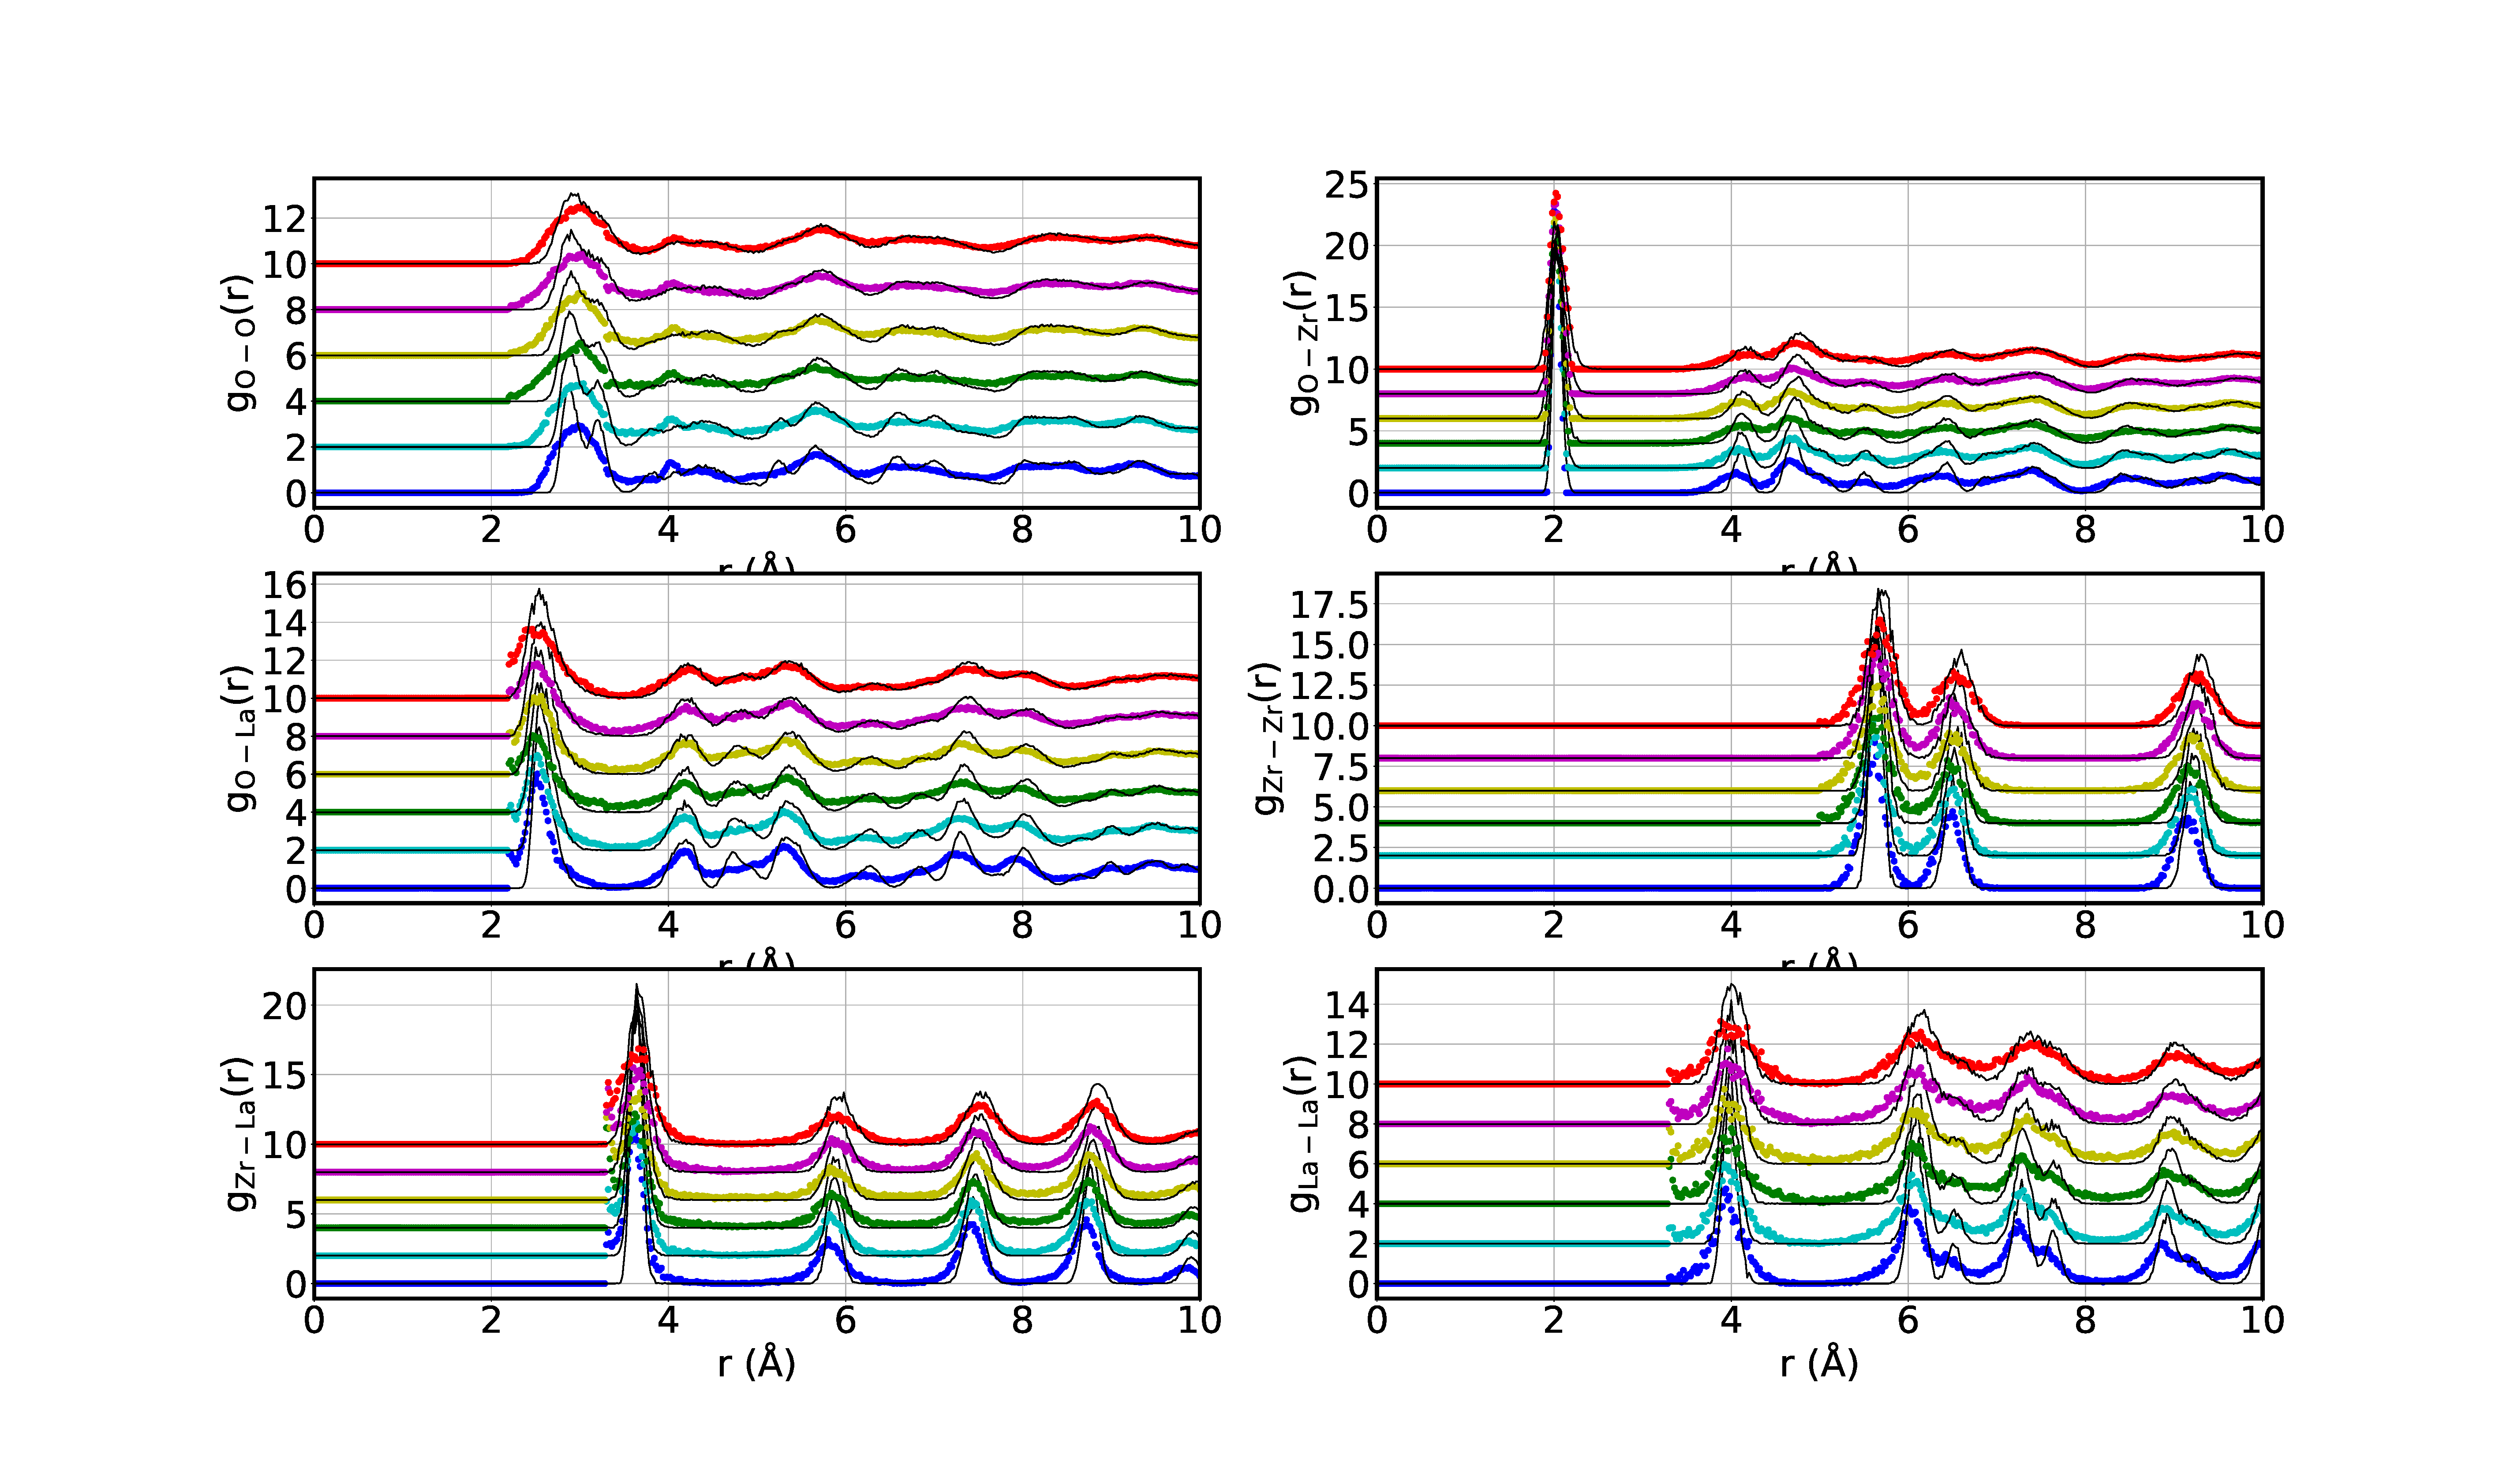
\includegraphics[width=0.5\textwidth]{Pics/partialPDFwithoutLi.pdf}
\caption{The distributions calculated from RMCProfile of (1) O-O;(2) O-Zr;(3) O-La; (4) Zr-Zr; (5) Zr-La; (6) La-La at low-$r$ range for all temperatures. A constant offset has been applied to separate those curves. The solid lines (black) indicate the values obtained from Molecular Dynamic simulation}
\label{fig:partialPDFwithoutLi}
\end{figure}


\subsection{Electrochemical Impedance Spectroscopy}

The EIS of the LLZO were examined with a in-plane geometry at elevated temperatures from -20$^oC$ to 100$^oC$, as shown in  Fig.\ref{fig:impedance}. 
From the Nyquist plots, a typical semi arc with the straight tail indicates the ion in-plane diffusion at low frequency occurs along the LLZO. 
The ion conductivity is about 2.1$\times$10$^{-4}$ S/cm at room temperature.

\begin{figure}
\centering
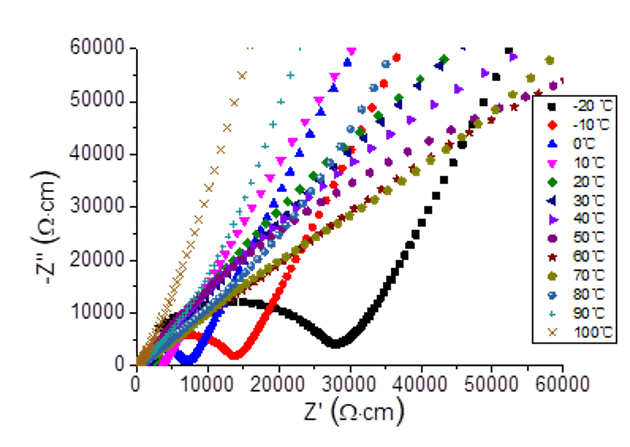
\includegraphics[width=0.5\textwidth]{Pics/impedance.png}
\caption{AC impedance data collected from -20$^oC$ to 100$^oC$.}
\label{fig:impedance}
\end{figure}

The activation energy can be calculated from the series of EIS at elevated temperatures shown in Fig.\ref{fig:arrhenius-plot}.
The activation energy E$_a$ is estimated based on the Arrhenius equation for the ionic conductivity

\begin{equation}
\sigma T = \sigma_0 e^{-E_a/k_B T}
\end{equation}


\begin{figure}
\centering

\includegraphics[width=0.5\textwidth]{Pics/arrhenius-plot.png}
\caption{A plot of conductivity as a function of temperature for LLZO. The line indicates an Arrhenius fit over the whole temperature range.}
\label{fig:arrhenius-plot}
\end{figure}

where $\sigma$ is the ionic conductivity, $\sigma_0$ is a pre-exponential factor, T is the absolute temperature, and k$_B$ is the Boltzmann constant. 
Furthermore, the diffusion coefficient was calculated using the Nernst-Einstein-equation

\begin{equation}
D=\frac{\sigma k_B T}{N_{Li} q^2}
\end{equation}

where q is the charge of the lithium and N$_{Li}$ the concentration of lithium, in this case for a cubic LLZO structure.
The calculated activation energy is about 0.36~eV which is in good agreement to other publications, 
as well as the diffusion coefficient shown in Fig.\ref{fig:DiffusionCoefficient} with 1.31 $\times$ 10$^{-13}$ m$^2$s$^{-1}$ at room temperature.  



\begin{figure}
\centering
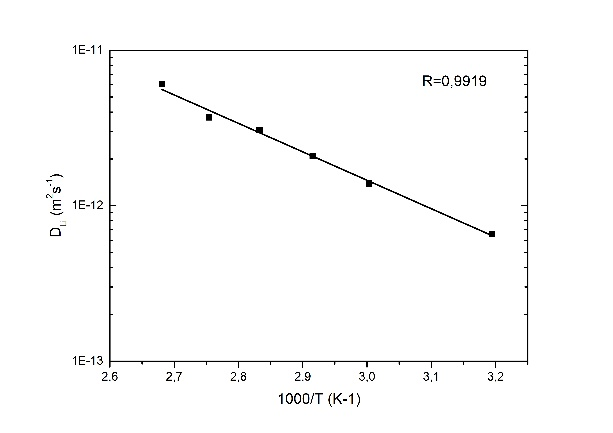
\includegraphics[width=0.5\textwidth]{Pics/DiffusionCoefficient.png}
\caption{Diffusion coefficient at different temperatures}
\label{fig:DiffusionCoefficient}
\end{figure}


\subsection{Lithium Distribution and Dynamics Analysis}



The 3D density maps of Li in cubic garnets are shown in Fig.\ref{fig:pdfs}.
The lithium distribution can ben expected in liquid and amorphous materials

\begin{figure*}
\centering
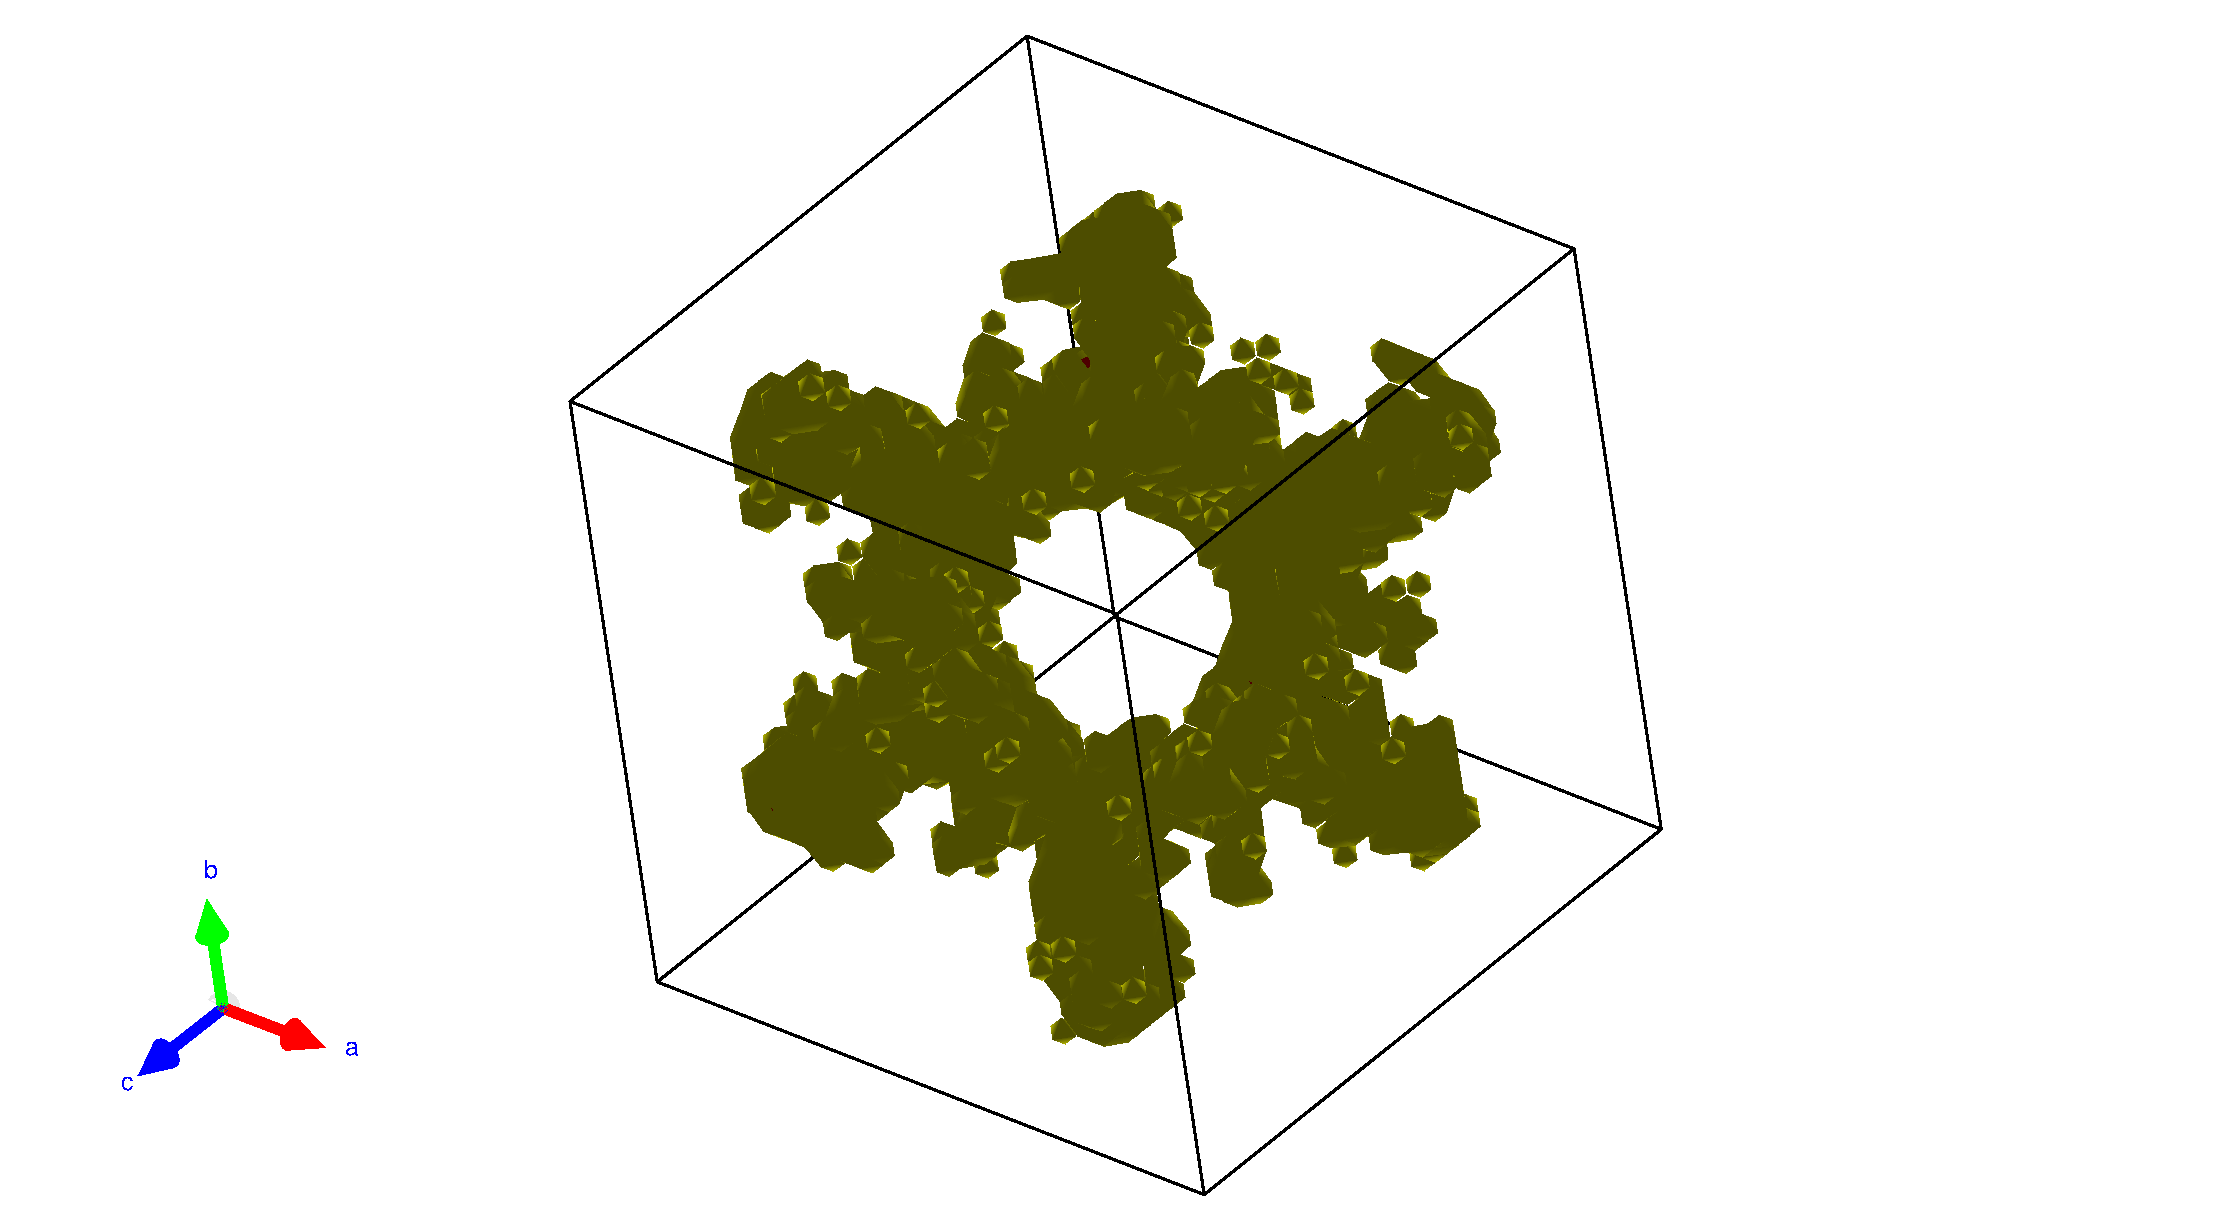
\includegraphics[width=0.9\textwidth]{Pics/pdfs.pdf}
\caption{Isosurfaces with level of 0.1~\AA$^{-3}$ (yellow) and 3~\AA$^{-3}$ (red)}
\label{fig:pdfs}
\end{figure*}

\begin{figure}
\centering
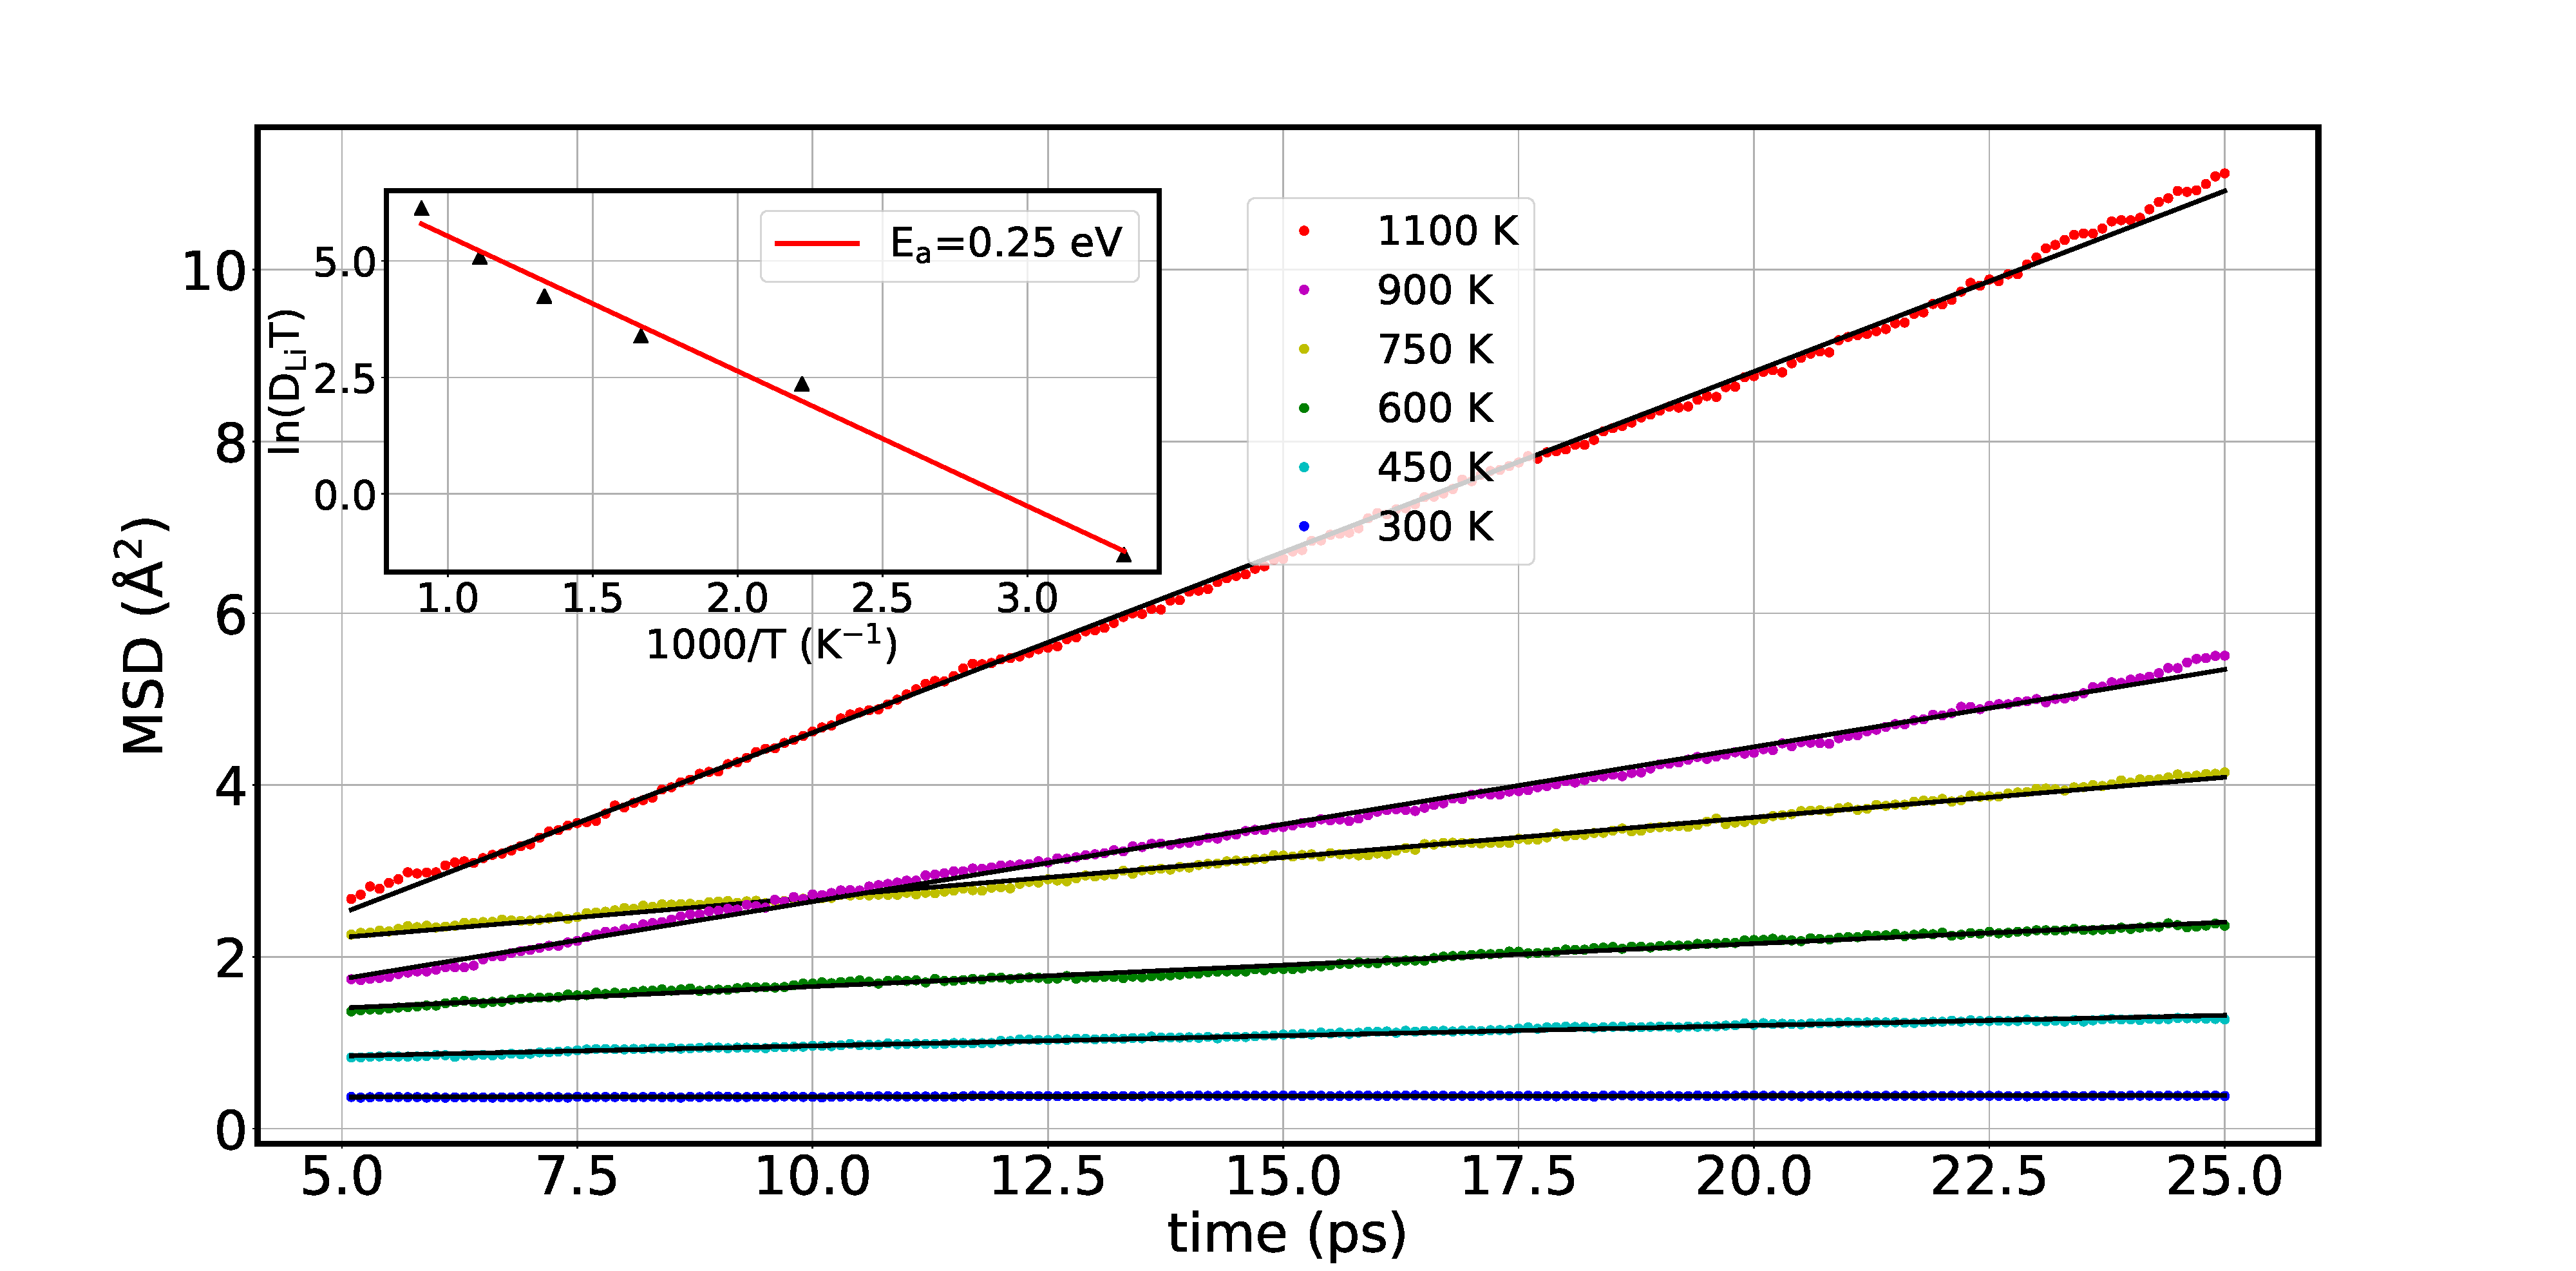
\includegraphics[width=0.5\textwidth]{Pics/MSD.pdf}
\caption{Mean squared displacement (MSD) of Li from 300 K to 1100 K.
The slope of MSD of each temperature data set yields the diffusion constant (D).
The inset shows a diffusion constant (D) versus temperatures.}
\label{fig:msd}
\end{figure}


%\begin{figure}
%\centering
%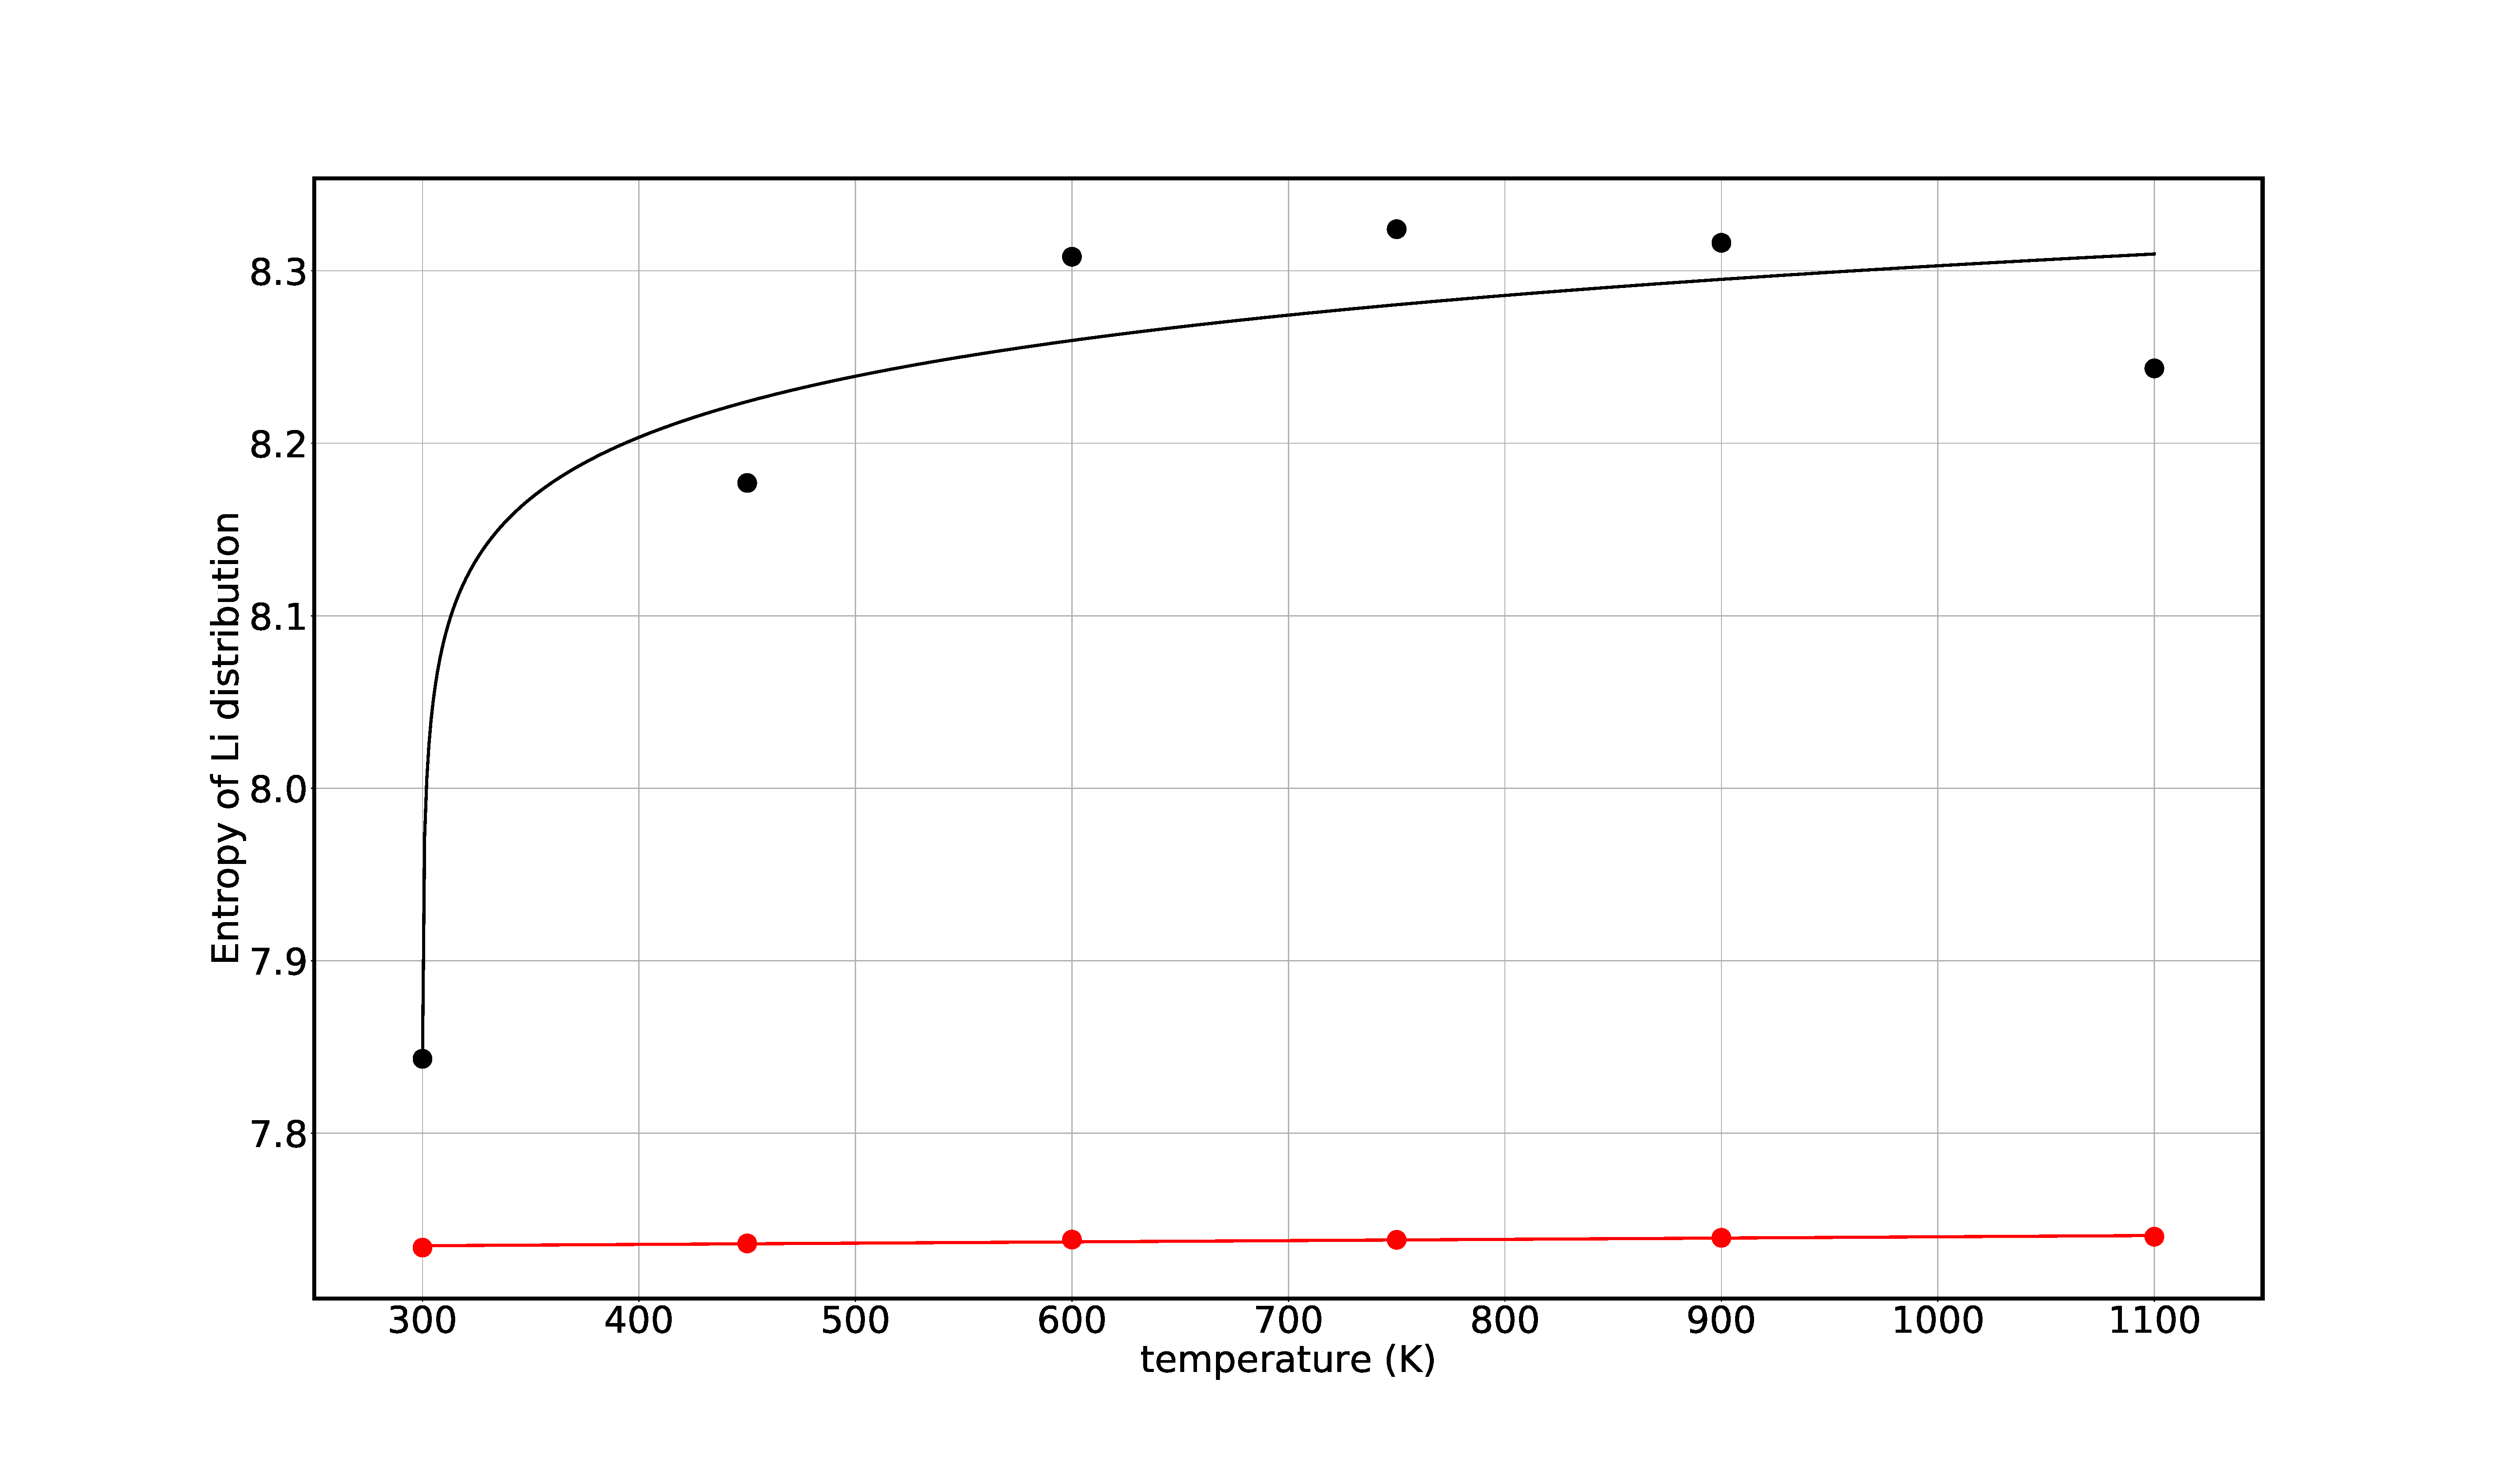
\includegraphics[width=0.5\textwidth]{Pics/entropy.pdf}
%\caption{The entropy of Li distribution. Data represented by back circles are the experimentally determined values using RMC refinement.
%Red circles represent the Molecular Dynamic simulation ones.}
%\label{fig:entropy}
%\end{figure}


%\begin{figure}
%\centering
%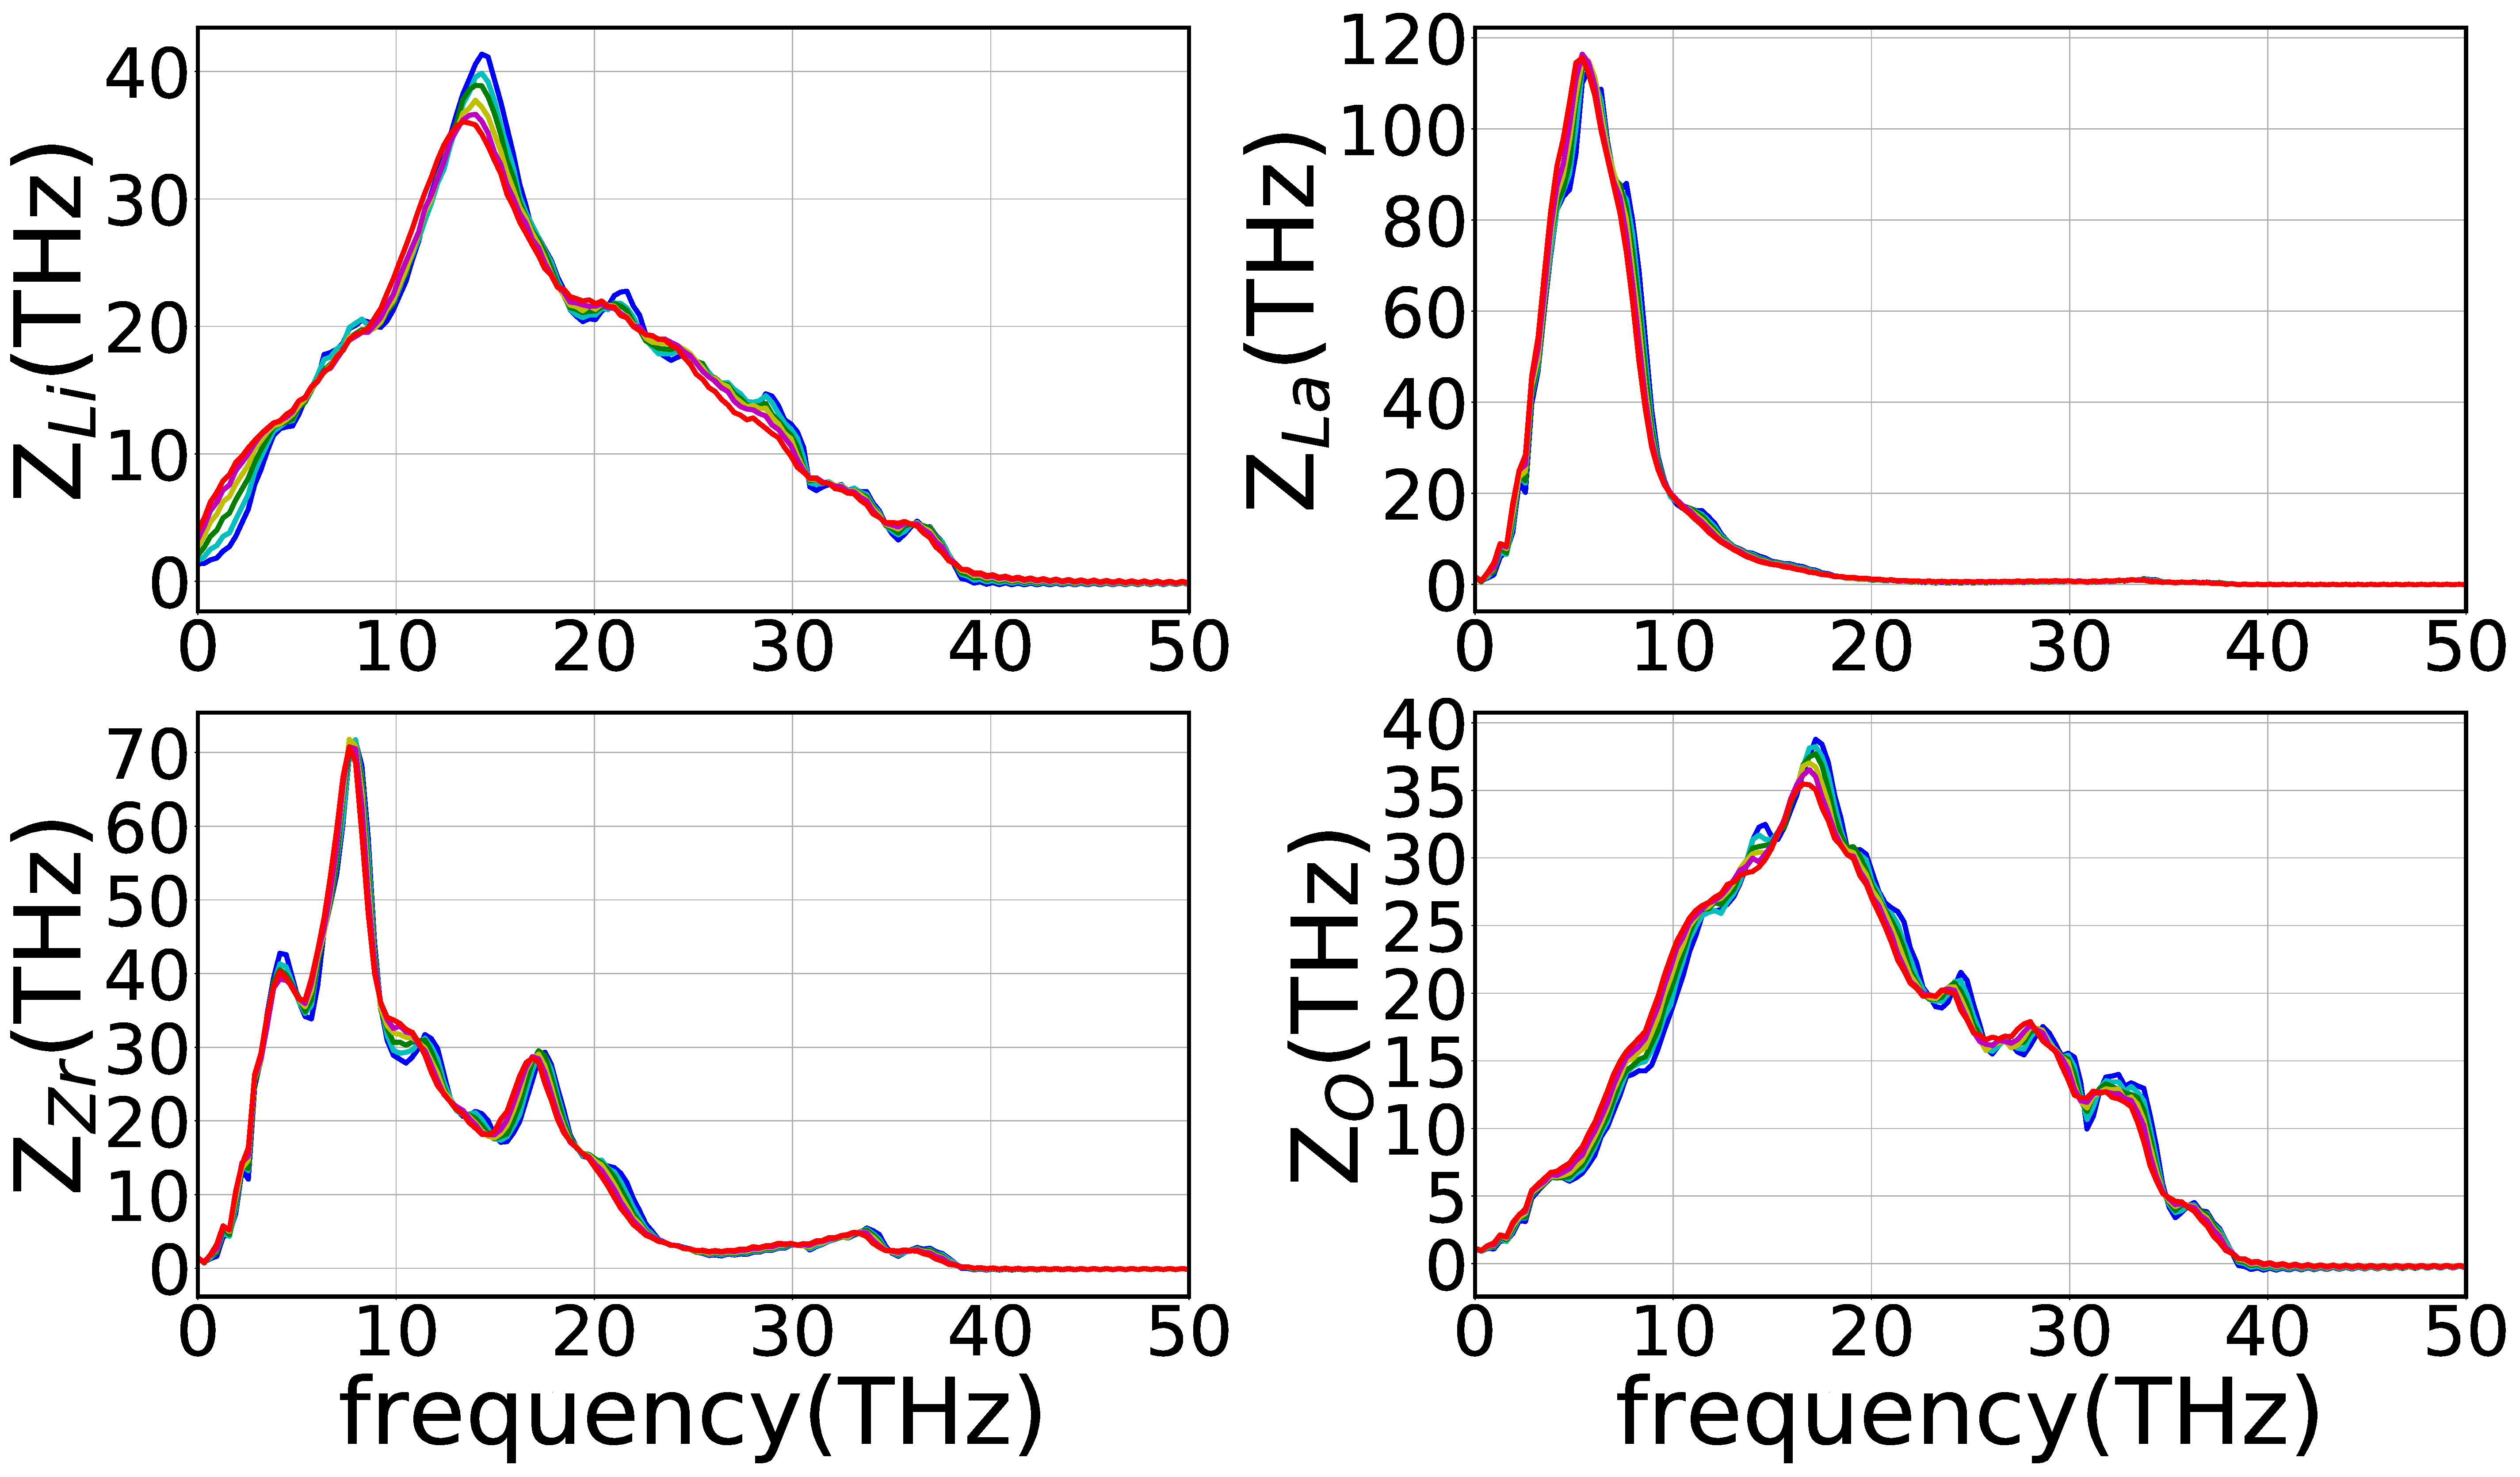
\includegraphics[width=0.5\textwidth]{Pics/powerSpectra.pdf}
%\caption{The power spectrum of Li vibrational frequencies.
% The zero point of power spectrum for each temperature yields the diffusion constant.
% The inset shows a diffusion constant (D) versus temperatures.}
%\label{fig:powerSpectra}
%\end{figure}


%\section{Simple model}\label{sec:model}
%
%\subsection{Description of the simple model}
%
%We have constructed a very simple model of the octahedral network, with sufficient interaction terms to reproduce the essential dynamics but few enough to give control of how the will behave. We consider composition AX$_3$, with corner-linked AX$_6$ octahedra. The first term is a Morse function to describe the change in separation $r$ of nearest-neighbour A--X bonds:
%\begin{equation}
%\label{eq:bond}
%E(r) = D \left[ \exp\left( - 2 \alpha (r - r_o) \right) - 2 \exp\left( - \alpha (r - r_o) \right) \right]
%\end{equation}
%This function has the advantage over a simple harmonic interaction that because it has anharmonicity it will give some thermal expansion of the A--X bond. Although there are three parameters, the zero-temperature distance $r_0$ simple sets a length scale. Given that we are not interested in the dissociation energy $D$ per se,
%the second differential evaluated at equilibrium, $E^{\prime \prime}_0 = 2 \alpha^2 D$, gives as the stretching frequency of the A--X bond and thus in practice we only need consider one parameter to be of interest. The parameter $D$ can be tuned to give the highest calculated vibrational frequency to be consistent with experimental measurements or ab initio calculations.
%
%The other two function concerns the bond angles. For the X--A--X angle of equilibrium value $90^\circ$, $\theta$, we use a potential energy function of the form
%\begin{equation}
%\label{eq:rightangle}
%E(\theta) = \tfrac{1}{2} k  \cos^2 \theta
%\end{equation}
%where $k$ is the force constant. For the linear A--X--A bond angle, $\phi$, we use a function of the form
%\begin{equation}
%E(\phi) = A (1 +  \cos \phi)
%\label{eq:linearangle}
%\end{equation}
%where $A$ is the force constant. This latter function has higher stability around $\phi = 180^\circ$. The value of the parameter $A$ give a non-zero frequency to the rigid unit modes. In principle $A$ could have negative values, which would cause a phase transition to a distorted state but one without complete order because all RUM distortions can condense simultaneously. The parameter $k$ controls the stiffness of the AX$_6$ octahedra. In the limit $k = 0$ we have a system of rigid bonds.
%
%Starting values of the force constants $D$, $\alpha$, $k$ and $A$ were estimated by calculating the phonon dispersion curves for ScF$_3$ with appropriate masses, and comparing with those calculated by DFT. Calculations were performed using the GULP code \cite{Gale:2003eo,Gale:1997iq}.  The value of $r_0 = 2.0125$~\AA\ was set as half the unit cell length of ScF$_3$, the value of $\alpha$ was arbitrarily set as 1.55~\AA$^{-1}$, The value of $D$ was set as 2.0~eV to math the highest frequency with that of ScF$_3$, the value of $A$ was set as 0.025~eV to give the rotational phonon frequency for wave vectors between the points M and R to be similar to that of ScF$_3$, and the value of $k$ was set as 1.5~eV to ensure that a matching of the frequencies of the transverse acoustic modes, which give rise to bending of the corresponding bond angle. The calculated dispersion curves are shown in Figure \ref{fig:dispersioncurves}. In this diagram we colour the dispersion curves according to the value of the mode Gr\"{u}neisen parameter following methods we have described previously \cite{Rimmer:2015km}. What is interesting is the extent to which the simple model reflects the DFT dispersion curves, both in overall shape and in the distribution of values, including sign, of mode Gr\"{u}neisen parameters. The main peculiarity of the model is that the elastic constant $C_{12} = 0$, far from the normal Cauchy relationship for cubic materials with central forces of $C_{12} = C_{44}$. This has little effect on the physical properties.
%
%\begin{figure}[t]
%\begin{center}
%\includegraphics[width=0.4\textwidth]{dispersion_curves.pdf}
%\caption{Calculated dispersion curves of ScF$_3$ based on the model indicated in equations \ref{eq:bond}--\ref{eq:linearangle}. The curves are coloured red or blue depending on the sign of the mode Gr\"{u}neisen parameter, as discussed in the text, with the intensity of the colour reflecting the size of the mode Gr\"{u}neisen parameter up to some saturation value. In this calculation $D = 2.0$~eV, $r_0 = 2.0125$~\AA, $\alpha = 1.55$~\AA$^{-1}$, $k = 1.5$~eV, and $A = 0.025$~eV.}
%\label{fig:dispersioncurves}
%\end{center}
%\end{figure}
%
%In principle this model contains all the essential interactions to give negative thermal expansion, a characteristic of ScF$_3$ and ReO$_3$ if not of many other perovskites other than when associated with a displacive phase transition or through magnetic/electronic effects.



\section{Conclusions}
The conclusions section should come in this section at the end of the article, before the Conflicts of interest statement.

\section{Appendix}

\subsection{The Correlation Functions}

Time-dependent correlation functions are valuable tools to describe the average way the quantity will change with time,
and predict the trends within the behaviour of atomic structure and dynamics.


One of the simplest correlation function for velocity with a mean value of zero, $C(t)$, is defined as
%x
 \begin{equation}
C(t)=\frac{\langle v(0)v(t)\rangle}{\langle | v(0)|^2 \rangle}
=\frac{(\lim \mathcal{T}\rightarrow \infty) \frac{1}{\mathcal{T}} \int^{\mathcal{T}}_{0} v(t')v(t+t')dt' }{\langle v^2 \rangle}
\end{equation}

For  the harmonic crystal, the velocity of the $j$-th atom is given as

\begin{equation}
v_j(t)=\frac{-i}{(Nm_j)^{1/2}}\sum_{\textbf{k},v}\omega(\textbf{k},v)\textbf{e}_j(\textbf{k},v)exp(i\textbf{k}\cdot \textbf{r})Q(\textbf{k},v,t)
\end{equation}

and leads to the classical result:
\begin{equation}
\sum_j  m_j \langle |v_j(t)\cdot v_j(0) |\rangle = \frac{k_B T}{N}\sum_{\textbf{K},v}\cos (\omega(\textbf{k}, v)t)
\end{equation}

In addition, the power spectra $Z(\omega)$ is given by the Fourier transform of $C(t)$:

\begin{equation}
Z(\omega)=\int C(t)exp(-i\omega t)dt
\end{equation}

It can be seen that the power spectrum of the mass-weighted velocity correlation function is equal to the phonon density of states.

Consider another correlation function for position of atom, $G_s(r,t)$, is defined as

\begin{align*}
G_s(\Delta r,t)&=\frac{\langle r(0)r(t)\rangle}{\langle | r(0)|^2 \rangle} \\
        &=\frac{1}{N}\sum_{j}^{N}\int \langle \delta(r'-r_j(0))\delta(r'+\Delta r -r_j(t))dr' \rangle \\
        &=\frac{1}{N}\langle \sum_{j}^{N}\delta(\Delta r +r_j(0)-r_j(t))\rangle
\end{align*}

which is related to the probability of finding an atom in the volume $dr$ at position $\Delta r$ for a time interval of $t$,
and can be named as self-part of van Hove correlation function.

The mean square displacement (MSD) $\langle \Delta r_i(t)\rangle ^2$  is a measure of the deviation of the position of an atom with
respect to a reference position over time. MSD is related to the $G_s(r,t)$ as:

\begin{equation}
  \langle \Delta r_i(t)\rangle ^2=\int_{0}^{\infty} (\Delta r_i(t))^2\cdot 4\pi(\Delta r_i(t))^2G_s(\Delta r,t)d\Delta r
\end{equation}

\subsection{ Nernst-Einstein  Equation}

The value of ionic conductivity ($\sigma$) is determined by the impedance spectroscopy.
In solid electrolytes, as the anions are immobile, the ionic conduction is driven by the diffusion of Li$^+$ ions.
The connection between the diffusion constant (D) and $\sigma$ is defined by the Nernst-Einstein (NE) equation,
which are widely used for electrolyte system. NE equation is given as

\begin{equation}
D(T)=\frac{kT}{Ne^2}\sigma(T)
\end{equation}

where $k$ is the Boltzmann constant, $e$ is the elementary charge, and N is the number of carrier ions.

\section*{Conflicts of interest}
There are no conflicts to declare.

\section*{Acknowledgements}
The Acknowledgements come at the end of an article after Conflicts of interest and before the Notes and references.

%%%END OF MAIN TEXT%%%

%The \balance command can be used to balance the columns on the final page if desired. It should be placed anywhere within the first column of the last page.

\balance

%If notes are included in your references you can change the title from 'References' to 'Notes and references' using the following command:
%\renewcommand\refname{Notes and references}

%%%REFERENCES%%%
\bibliography{rsc} %You need to replace "rsc" on this line with the name of your .bib file
\bibliographystyle{rsc} %the RSC's .bst file

\end{document}
